\subsection{Diseños finales}

\subsubsection{Diagrama de clases definitivo}
Presentamos ahora el diagrama de clases completo y definitivo  de nuestra solución. 
Lo mostramos separado en 3 partes que juntos hacen al total del diagrama. \\

\begin{figure}[H]
\centering
\caption{Diagrama de clases: clases del yacimiento}
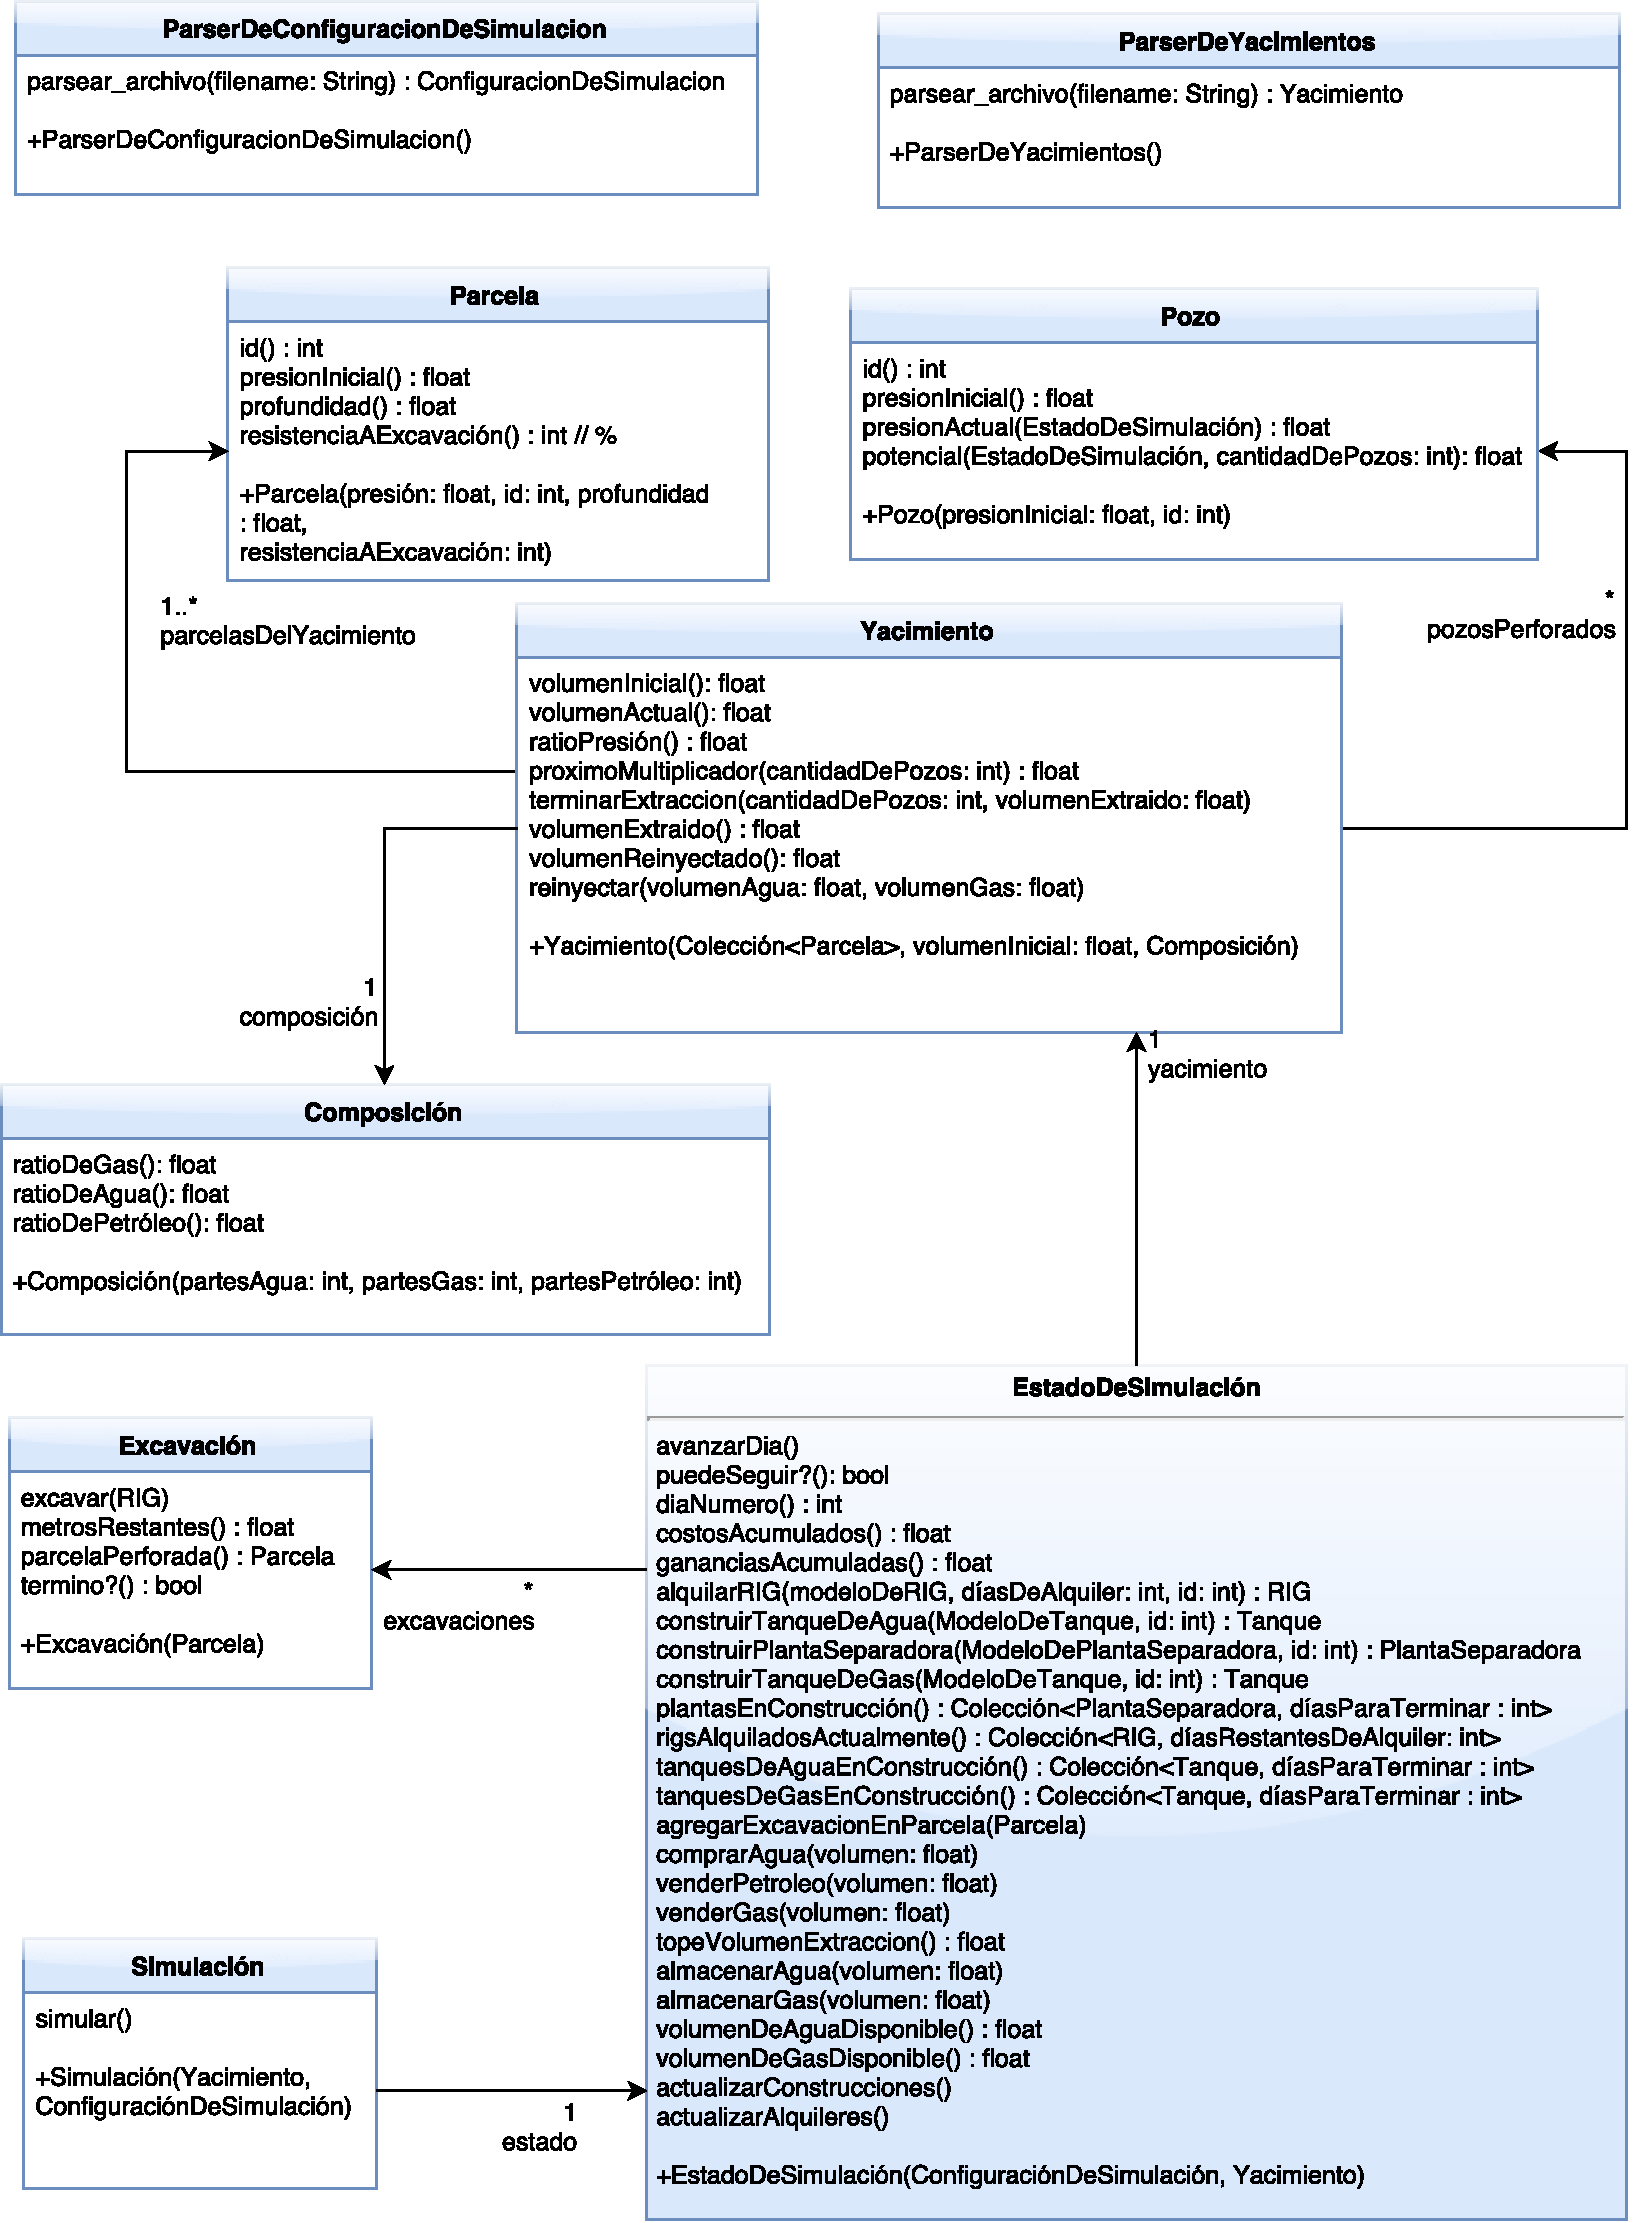
\includegraphics[width=0.95\textwidth, keepaspectratio]{clases-yacimiento}
\end{figure}

\newpage
\begin{figure}[H]
\centering
\caption{Diagrama de clases: clases de tanques, plantas separadoras y RIGS}
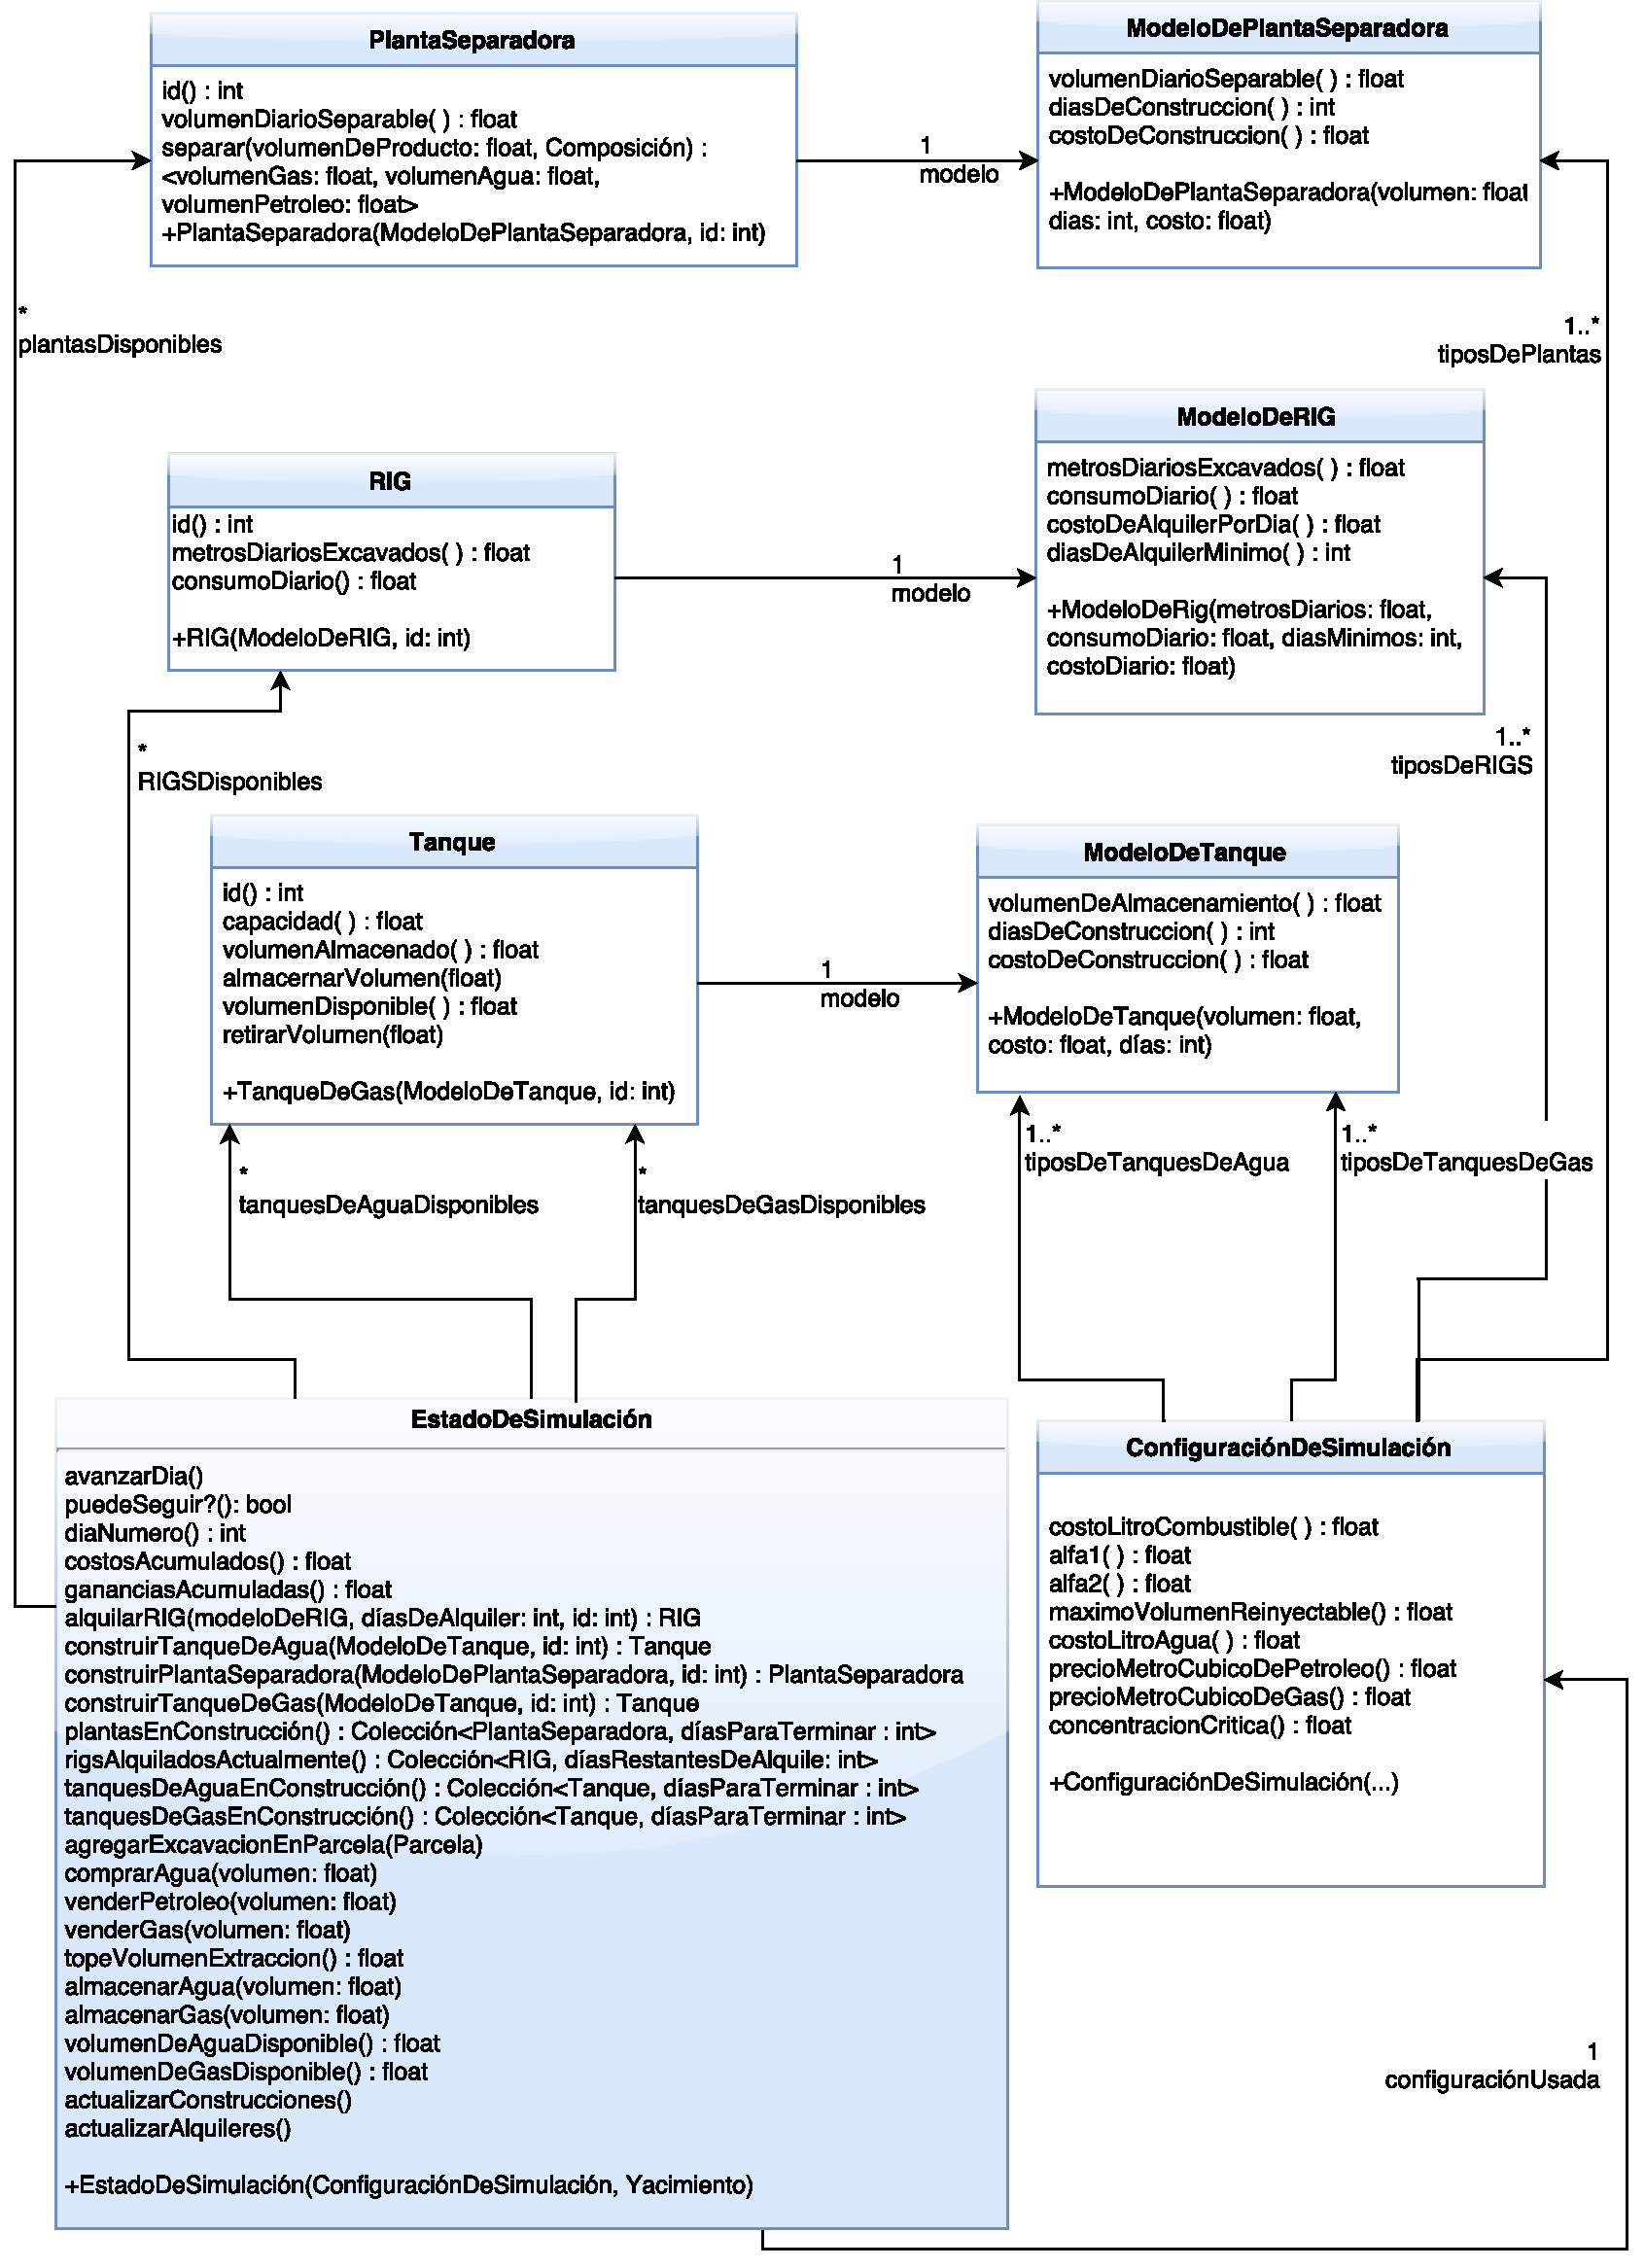
\includegraphics[width=0.95\textwidth, keepaspectratio]{clases-tanques-plantas}
\end{figure}

\newpage
\begin{figure}[H]
\centering
\caption{Diagrama de clases: clases de criterios del grupo de ingeniería}
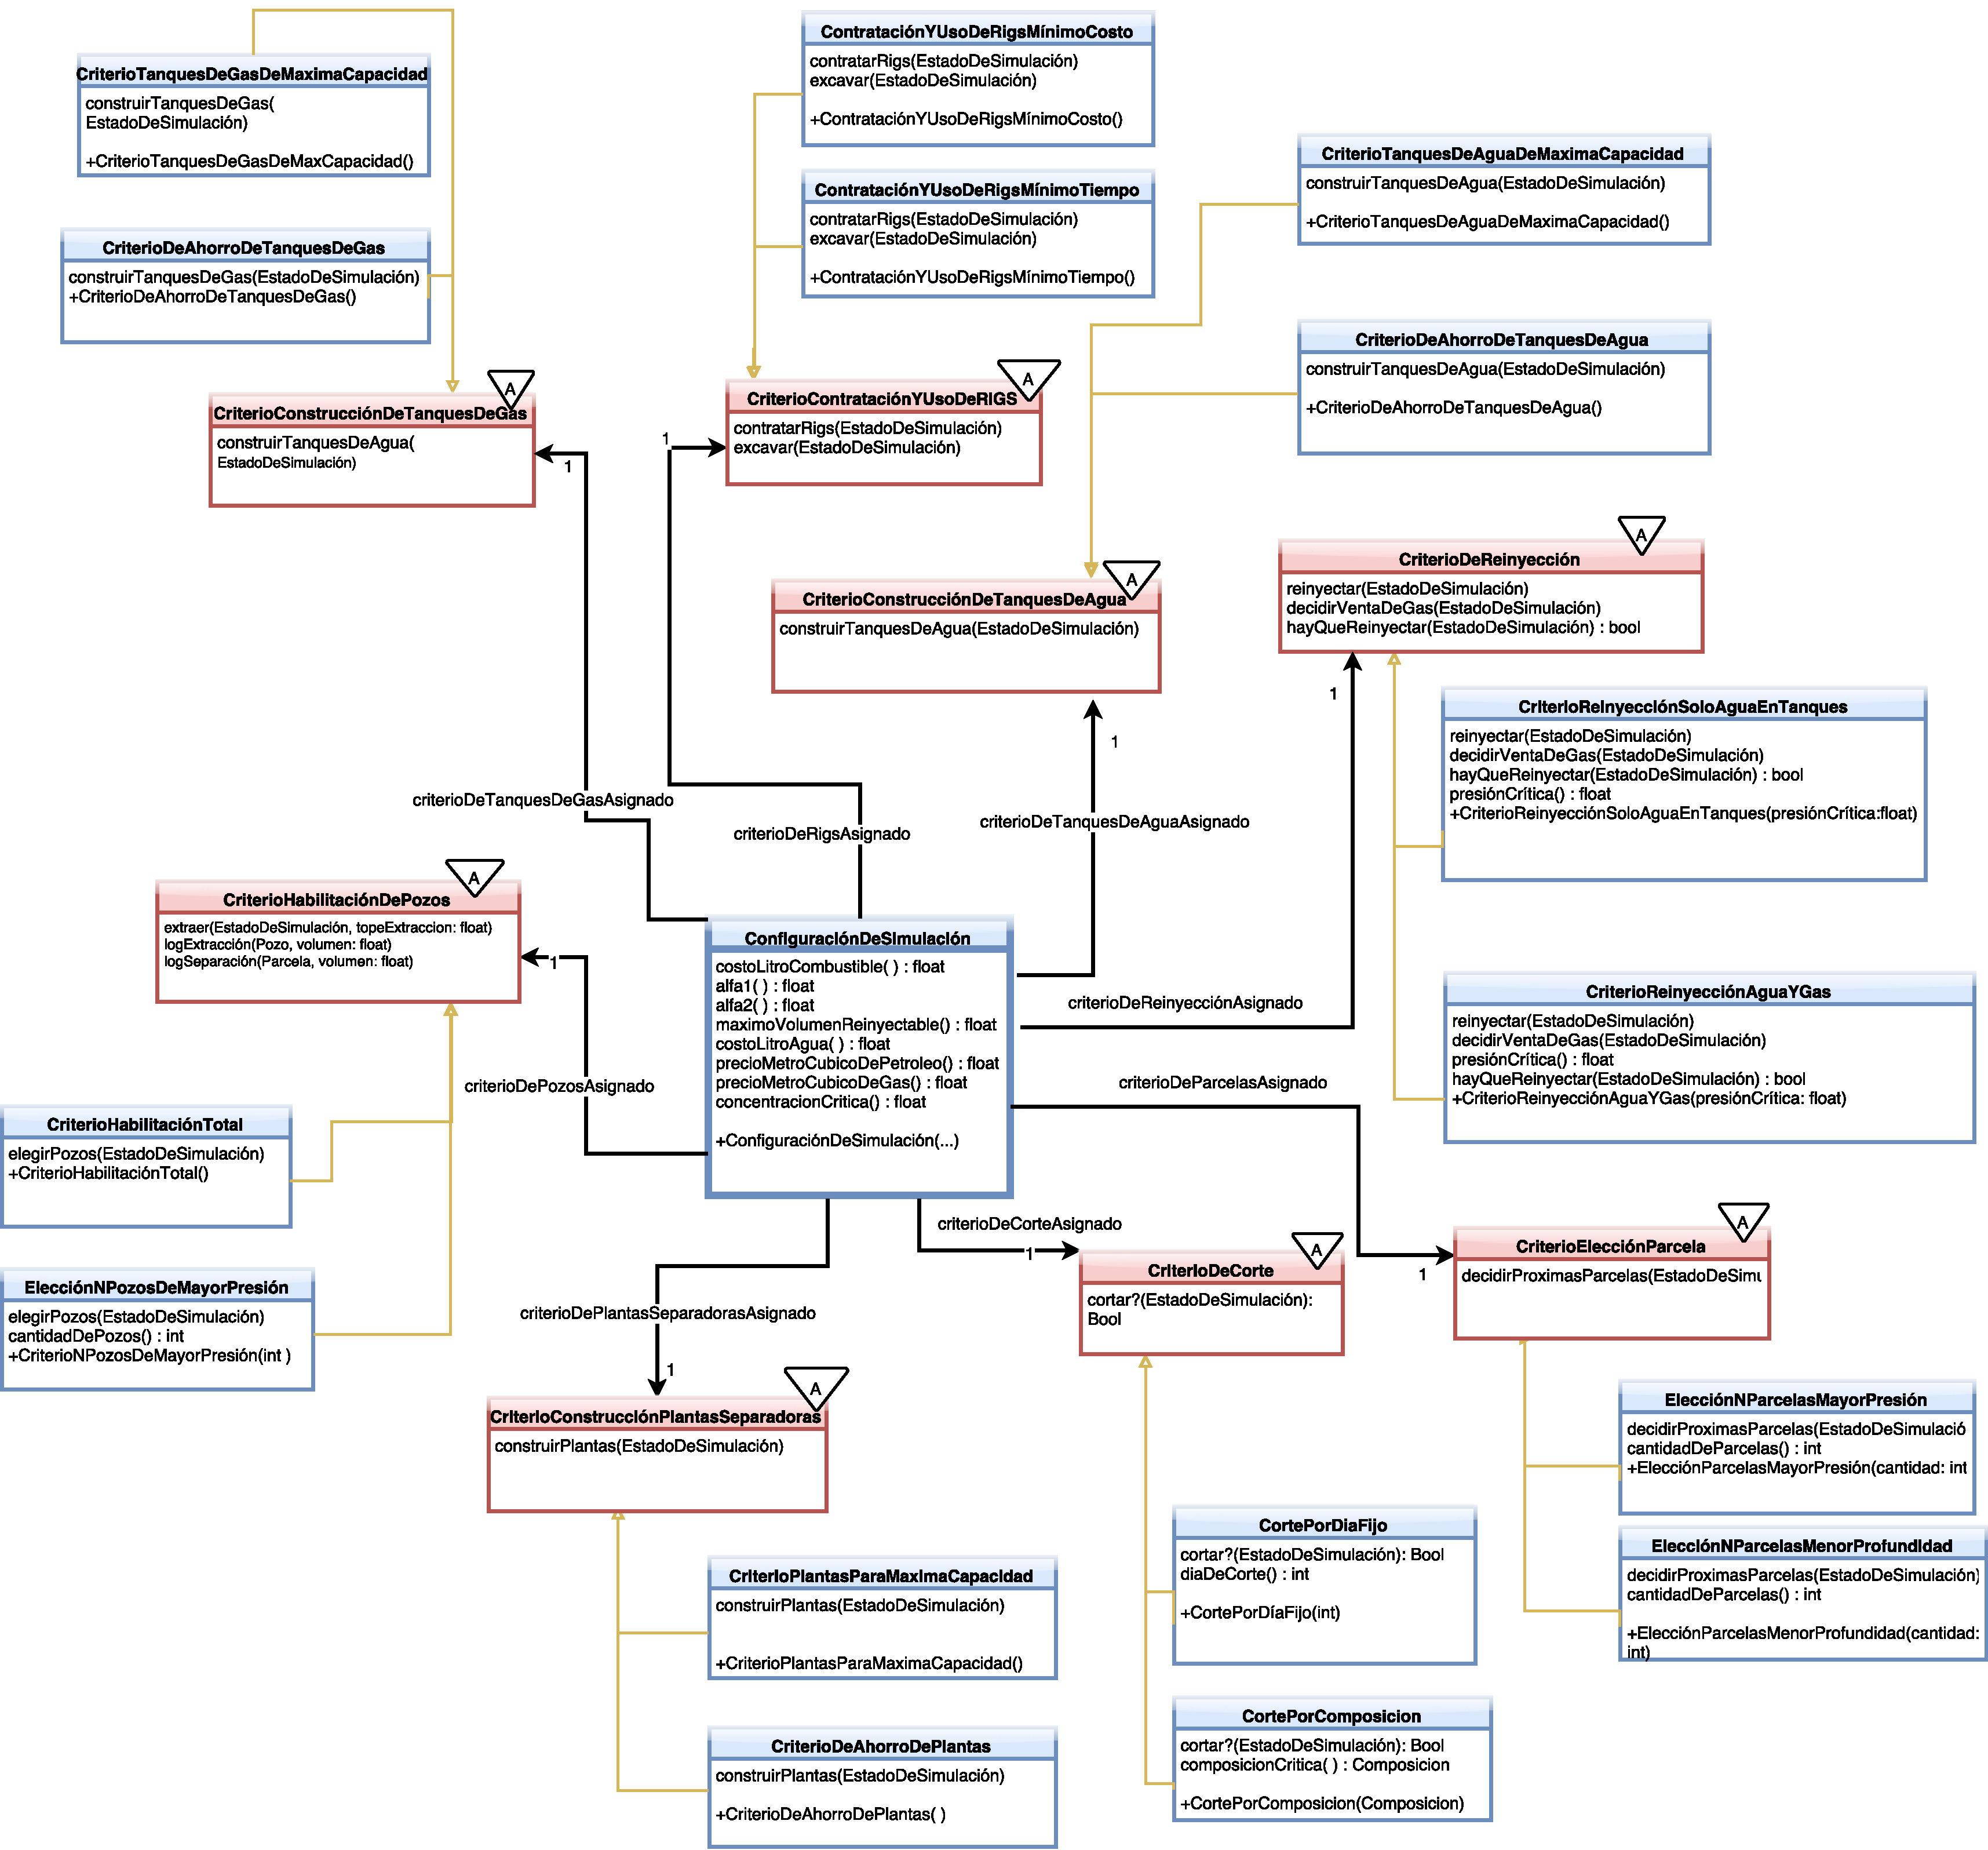
\includegraphics[width=1.10\textwidth, keepaspectratio]{clases-criterios}
\end{figure}

%%% desarrollo / explicacion 
Pueden apreciarse algunas diferencias entre el diagrama completo y las primeras 
ideas planteadas.

Por ejemplo, ahora el simulador no es el objeto central sino que simplemente es un cliente del EstadoDeSimulación, el cual sí ocupa dicho lugar central. 

Si bien se sigue con la idea de delegar decisiones a las clases de los criterios, el estado ahora no las conoce de primera mano, sino que estas son conocidas por una clase intermedia que representa la configuración de la simulación. 

Dicha clase actúa como un repositorio de los parámetros ingresados a la simulación. De esta manera el único eje de cambio del estado refiere a aspectos propios de la logística del día a día de la simulación (responder a alquileres, construcciones, ventas, etc), significando mayor cohesión.
\\

Los \emph{assets} (o recursos) de la simulación conocen un modelo y es a él a quien delegan los mensajes referentes a sus cualidades ``de fábrica''. Es responsabilidad de los criterios ir contando los números de id de sus construcciones y alquileres. Una alternativa a esto era consultarlos a la clase estado o que esta se encargara de ir contando cuando se le envían los mensajes de alquiler y construcción, pero nos pareció que no violaba la esencia de los criterios que se encargaran ellos mismos. 

Decidimos que modelar los tanques de agua y gas con una única clase, dado que es en su finalidad donde difieren. Responden a los mismos mensajes de la misma manera. Esto se asemeja a la realidad donde cisternas son utilizadas para almacenar diversos componentes.
\\

En un principio habíamos asociado cada pozo a su respectiva parcela, dado que en el mundo real \emph{los pozos están en las parcelas}, pero en el contexto de la simulación dicha asociación no aporta información y es irrelevante.
\\

Si bien podríamos haber hecho que la presión actual de un pozo fuera algo conocido por el mismo en todo momento y sea modificado día a día, decidimos que sea relativa al estado de la simulación. Esto se hace aprovechando el espíritu recursivo de las fórmulas de presión donde continuamente se multiplican valores sobre la presión inicial, dichos valores no dependen del pozo. 

Por lo tanto, el yacimiento conoce su \emph{ratioPresión} que representa las \emph{capas de multiplicación} de la fórmula recursiva, es decir, conserva el producto de todas las actualizaciones anteriores. Cuando se llama a \emph{presiónActual} de un pozo dado un estado, se multiplica la presión inicial por el ratio. Y día a día únicamente se actualiza el ratio multiplicándolo por $e^{-\beta_i}$ con $\beta_i$ definida como está en el enunciado.

Esto nos permite, en particular, que los pozos tengan esencia inmutable y que su presion esté ligada a un momento en particular de la simulación.
\\

La clase excavación representa parcelas en estado de perforación. Día  a día se actualizan los metros restantes hasta que llegan a 0, se anula la excavación y se agrega un nuevo pozo al yacimiento.
\\

Si bien no aporta información por ser una clase conocido por todos, existe tácitamente una clase logging que aporta el mensaje \emph{info} necesario para que el sistema pueda declarar, cuando haga falta, las acciones que se realizan. 
\\

En total, estos son todas las decisiones del equipo de ingeniería para las cuales 
desarrollamos \textbf{criterios} en forma de clases abstractas: 
\begin{itemize}
\item Elección de parcelas para excavación de pozos
\item Contratación de RIGS
\item Habilitación de pozos para extracción de producto
\item Construcción de plantas separadoras de producto
\item Construcción de tanques de agua
\item Construcción de tanques de gas
\item Reinyección 
\item Corte de explotación
\end{itemize}

Para cada uno de estos items, existe una clase correspondiente en nuestro modelo, 
cada una con un par de alternativas de estrategias. \\

Para los criterios que deciden construcciones, excavaciones o alquileres, decidimos implementar estrategias que decidan únicamente el primer día todo lo necesario para el resto de la explotación. Siendo criterios \emph{dummy} el resto de los días. \\

En la sección siguiente mostramos y explicamos algunos diagramas de secuencia 
de distintas partes del simulador, para entender mejor el funcionamiento interno 
del mismo y cómo nuestro diseño queda implementado finalmente. 

%%%%%%%%%%%%%%%%%%%%%%%%%%%%%%%%%%%%%%%%%%%%%%%%%
%%%%%%%%%%%%%%%%%%%%%%%%%%%%%%%%%%%%%%%%%%%%%%%%%
%%%%%%%%%%%%%%%%%%%%%%%%%%%%%%%%%%%%%%%%%%%%%%%%%

\newpage
\subsubsection{Diagramas de secuencia}
\textbf{Diagrama de avanzarDia}
\begin{figure}[H]
\centering
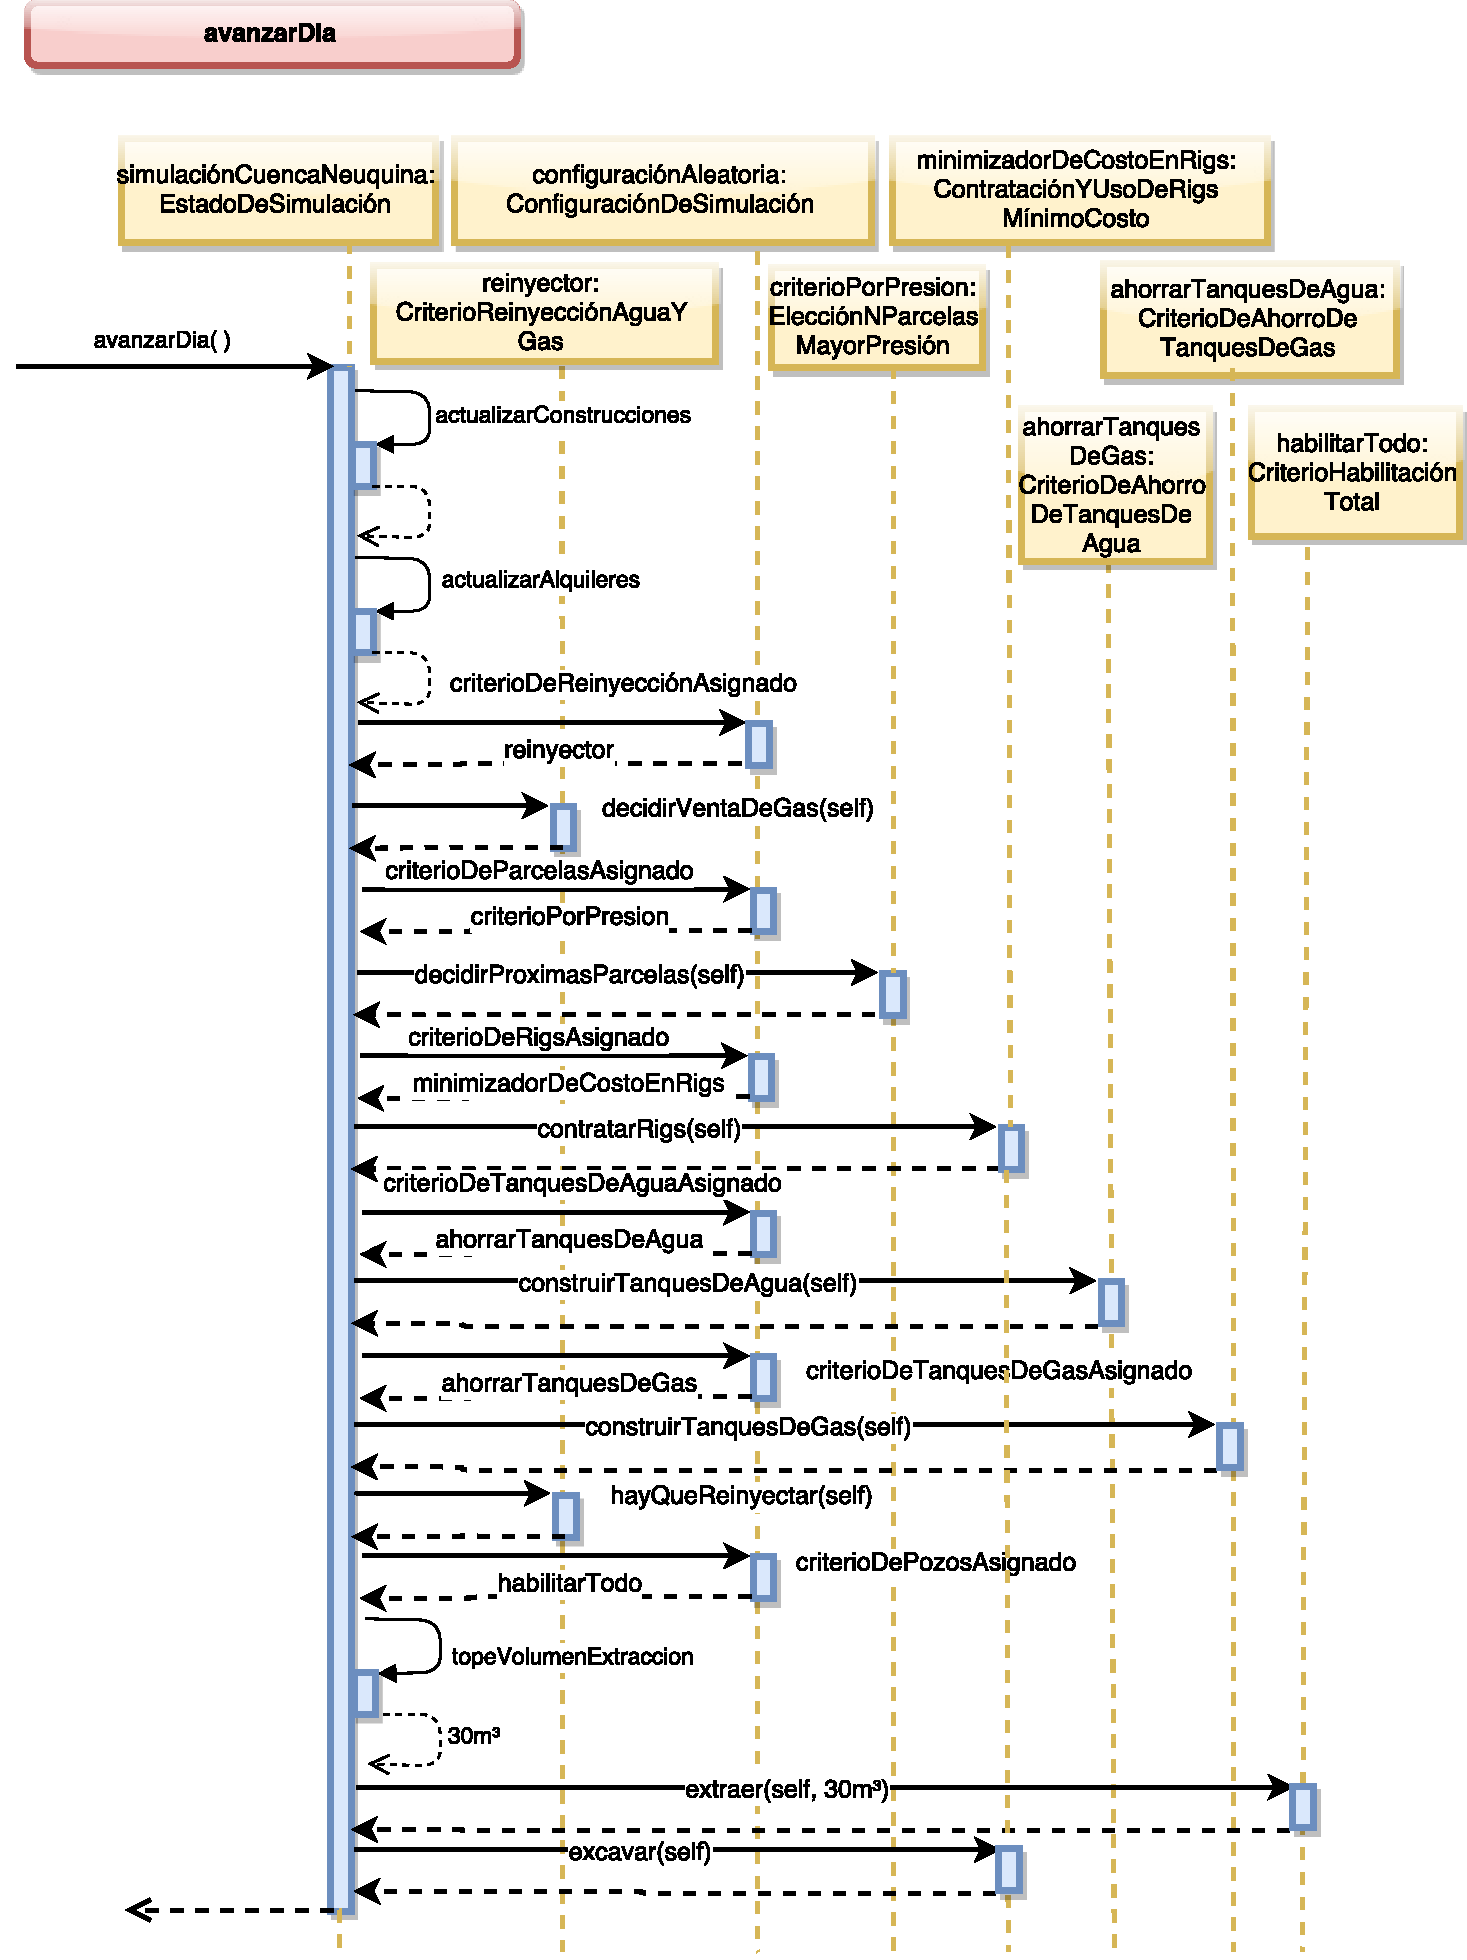
\includegraphics[width=1\textwidth, keepaspectratio]{avanzardia}
\end{figure}
La dinámica de la simulación está centrada en el mensaje \texttt{avanzarDia} del \texttt{EstadoDeSimulación}. Durante dicho mensaje, el estado se encarga de iniciar colaboraciones con todos los criterios para que se encarguen de hacer todos los cambios necesarios para desarrollar las funcionalidades del simulador (por ejemplo, 
empezar excavaciones, construcciones, habilitar pozos para extraer producto). 
\\

De esta manera, el estado se encarga únicamente de actualizar el día y los tiempos restantes de las construcciones y alquileres (y haciendo lo necesario en caso de que terminen). Los demás cambios en el sistema los comandan los criterios elegidos, en conocimiento del estado. Esto tiene sentido, dado que son las decisiones del día a día del equipo de ingeniería las que determinan el flujo y resultado de la simulación.
\\

\newpage
\textbf{Diagrama de secuencia de distintos tipos de criterios}

A continuación detallaremos con diagramas de secuencia algunas de las decisiones y colaboraciones que realizan los criterios definidos.
\\
%%%%%%%%%%%%%%%%%%%%%%%%%%%%%%%%%%%%%%%%%%%%%%%%%

\textbf{Diagrama de criterio de corte}
\begin{figure}[H]
\centering
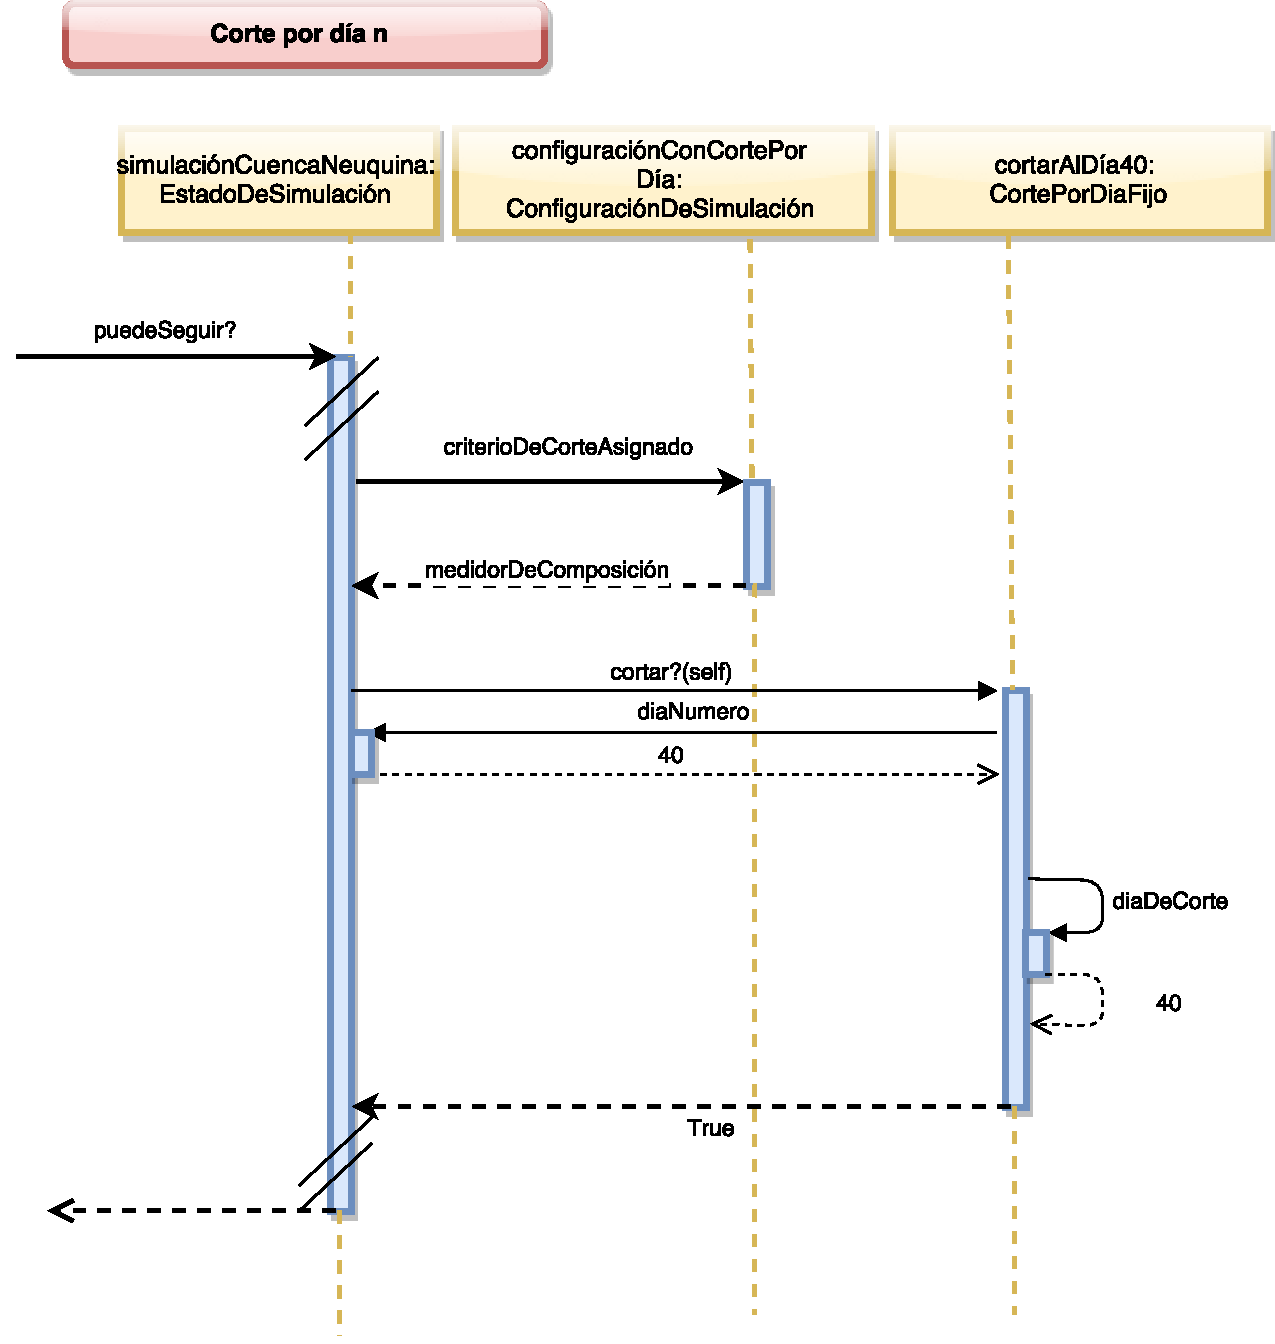
\includegraphics[width=1\textwidth, keepaspectratio]{corte}
\end{figure}

Durante la simulación, la clase \texttt{Simulación} se encarga constantemente 
de preguntarle al estado si debe continuar la simulación, mediante el mensaje 
\texttt{puedeSeguir?}. En caso de retornar \texttt{True}, la simulación 
le envía el mensaje \texttt{avanzarDía} al estado. 

Para el estado poder responder a esto, compara la proporción de petróleo en el 
yacimiento con el umbral mínimo permitido, y además utiliza su criterio de corte. 
Los criterios de corte solo están obligados a responder el 
mensaje \texttt{cortar?}. 

Este diagrama presenta un escenario en el cual el estado recibe el mensaje \texttt{puedeSeguir?}. En este caso, el criterio de corte por día fijo, en particular, 40. Por lo tanto el criterio decide que es necesario cortar. 

En el caso de un corte únicamente por composición, el criterio compararía a su vez también su propia composición crítica con la composición actual del yacimiento.

%%%%%%%%%%%%%%%%%%%%%%%%%%%%%%%%%%%%%%%%%%%%%%%%%

\newpage
\textbf{Diagrama de criterio de reinyección}
\begin{figure}[H]
\centering
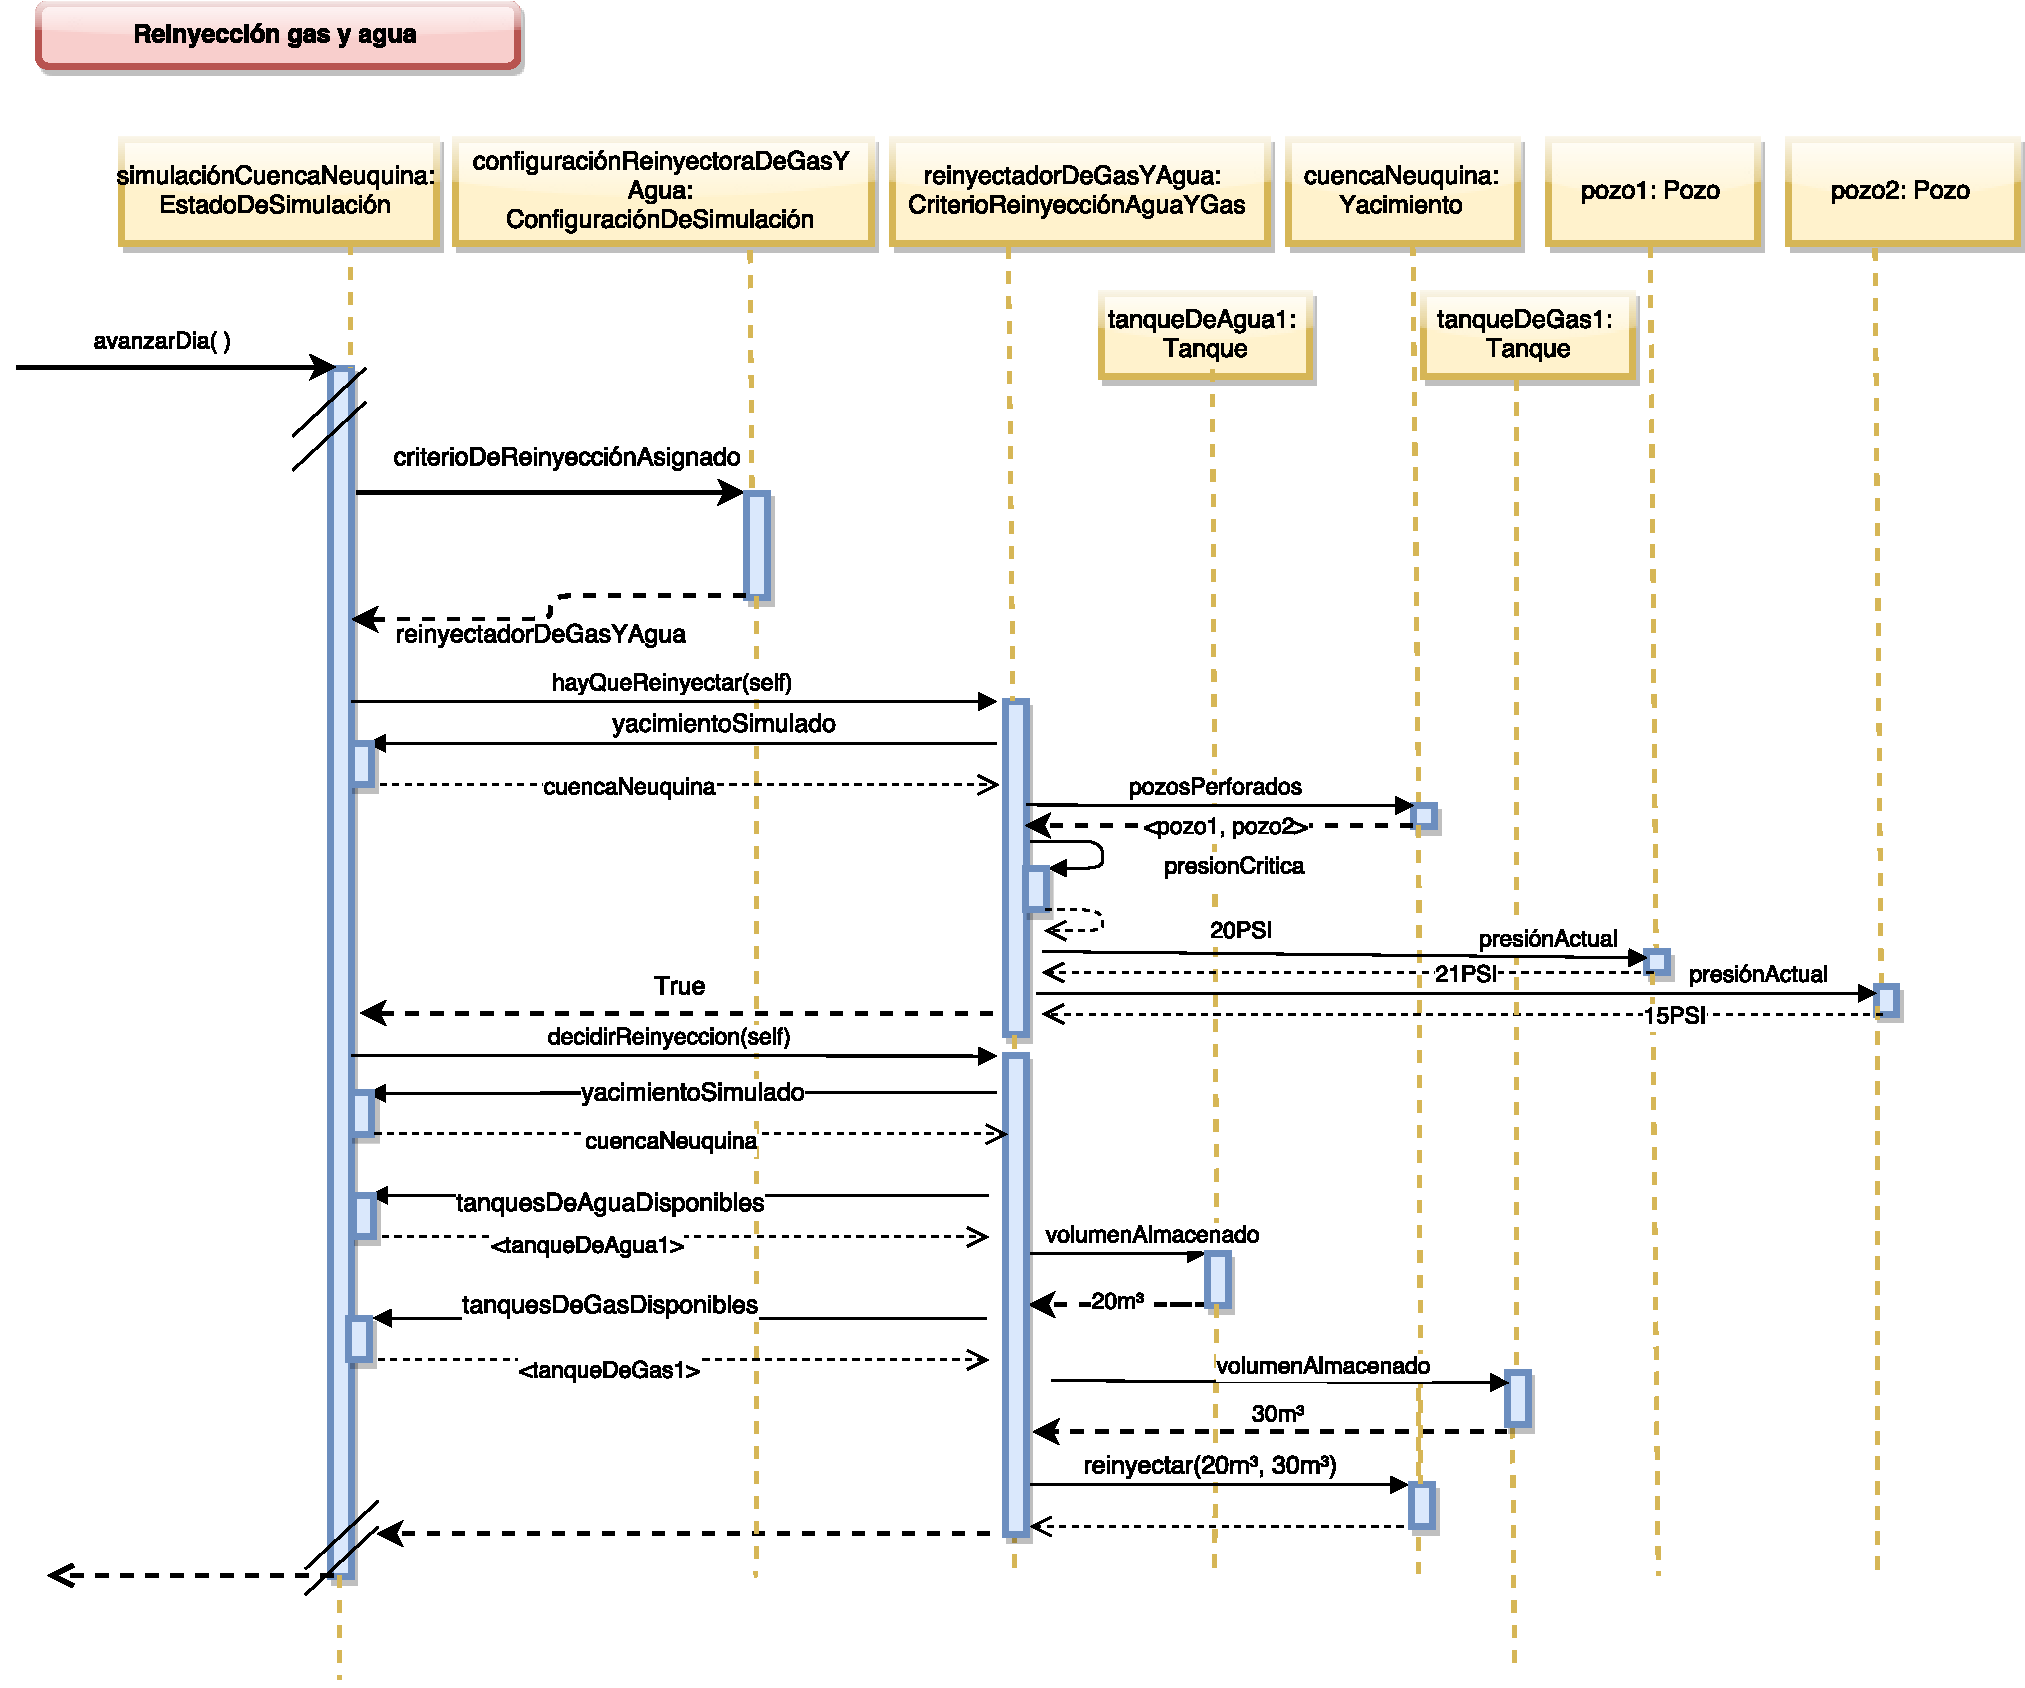
\includegraphics[width=1.15\textwidth, keepaspectratio]{reinyeccion}
\end{figure}

Dentro de \texttt{avanzarDía} del estado de simulación, se utiliza el criterio de 
reinyección seleccionado. Los criterios de reinyección deben saber responder a 3 
mensajes: \texttt{decidirVentaGas}, \texttt{hayQueReinyectar} y 
\texttt{reiyectar}. 


El escenario de la reinyección trata de una simulación configurada para reinyectar tanto gas como agua almacenada (nunca compra). Como el criterio reinyecta todo el agua y gas disponibles en tanques, al contar con un único tanque de cada tipo reinyecta su volumen almacenado. 
\\

El criterio decide reinyectar al recibir el mensaje \texttt{hayQueReinyectar} al notar que existe al menos un pozo con presión menor que la presión umbral seteada.
\\

Si bien al momento de reinyectar usa todo el gas, el criterio implementa el mensaje \texttt{venderGas} de modo que guarde la mitad para las reinyecciones. En el caso del criterio de reinyección de solo agua almacenada, el gas es vendido en su totalidad, y las colaboraciones para reinyectar son las mismas pero obviando la consulta a tanques de gas. 

%%%%%%%%%%%%%%%%%%%%%%%%%%%%%%%%%%%%%%%%%%%%%%%%%

\newpage
\textbf{Diagrama de criterio de construcción de plantas}
\begin{figure}[H]
\centering
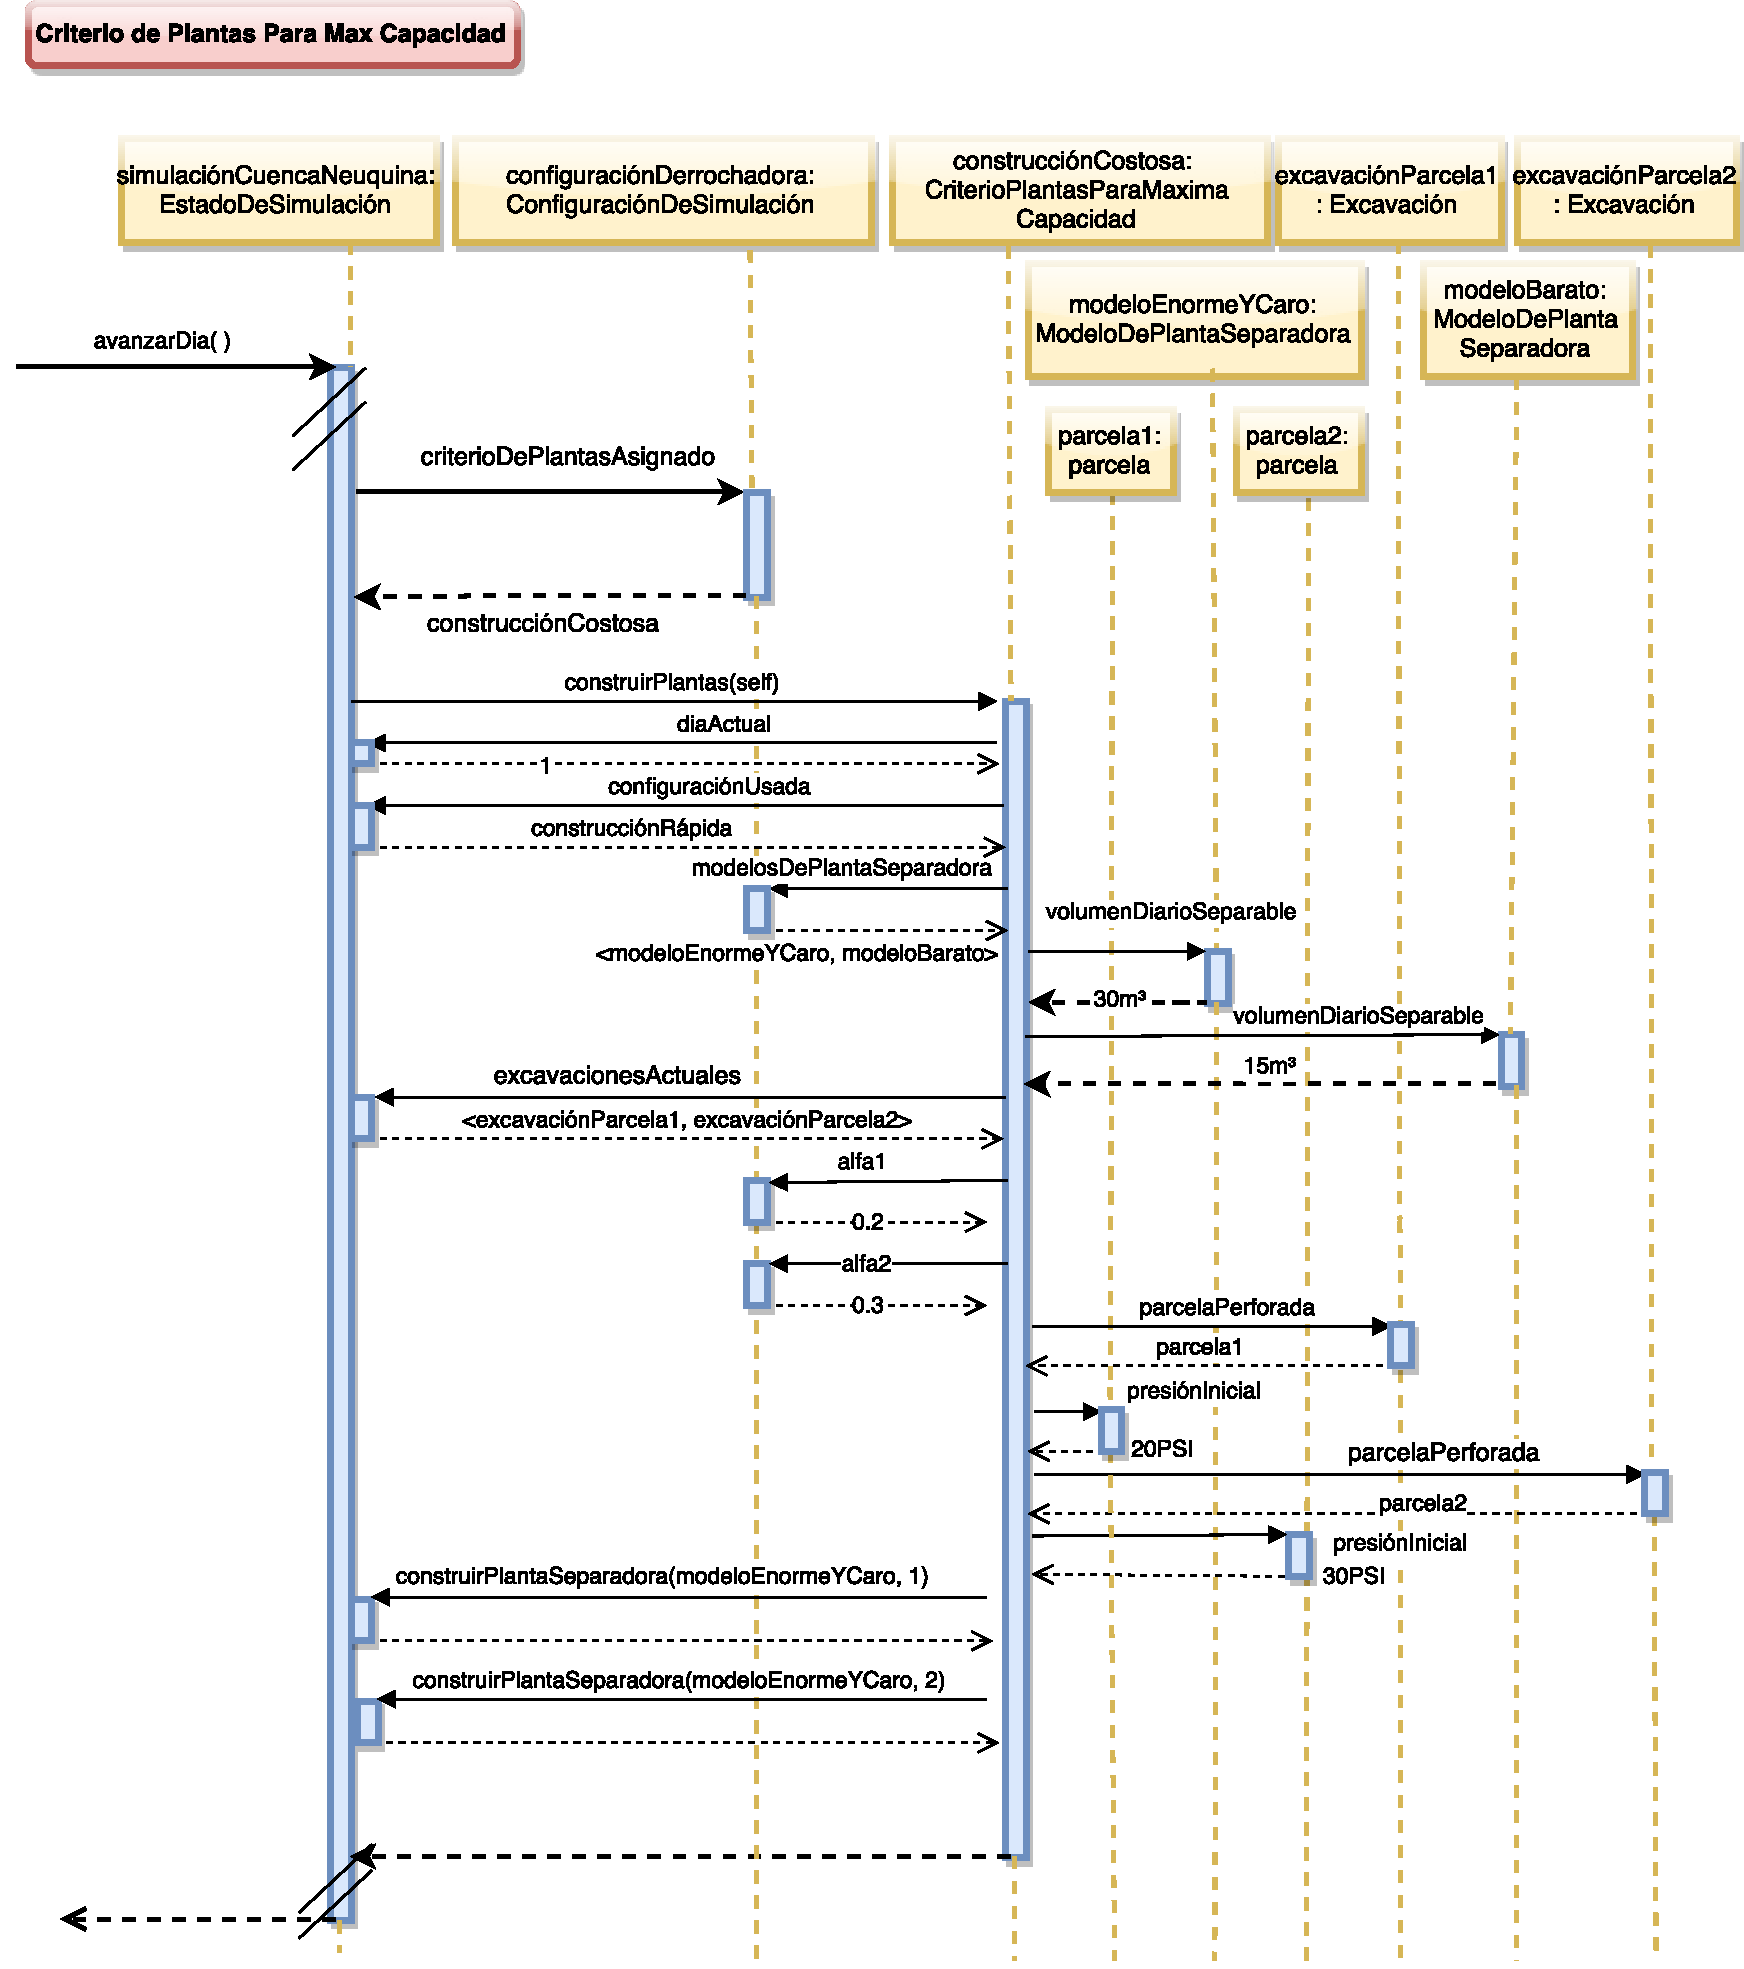
\includegraphics[width=1.15\textwidth, keepaspectratio]{plantas}
\end{figure}

En este diagrama el estado le delega al criterio constructor de plantas de la configuración la construcción de las mismas. Por tratarse de un criterio para máxima capacidad, el criterio calcula y construye la cantidad de plantas del modelo con mayor volumen diario separable necesarias para soportar el volumen extraído en todos los pozos en excavación el primer día de su funcionamiento. En este caso el criterio construye dos plantas del modelo más grande (también más costoso, como sería de esperar) tras haber consultado la presión inicial de las parcelas excavadas y los coeficientes de la configuración para calcular el volumen extraíble al primer día.
\\

El criterio de ahorro hace lo mismo pero solamente construye considerando la mitad de todo el producto extraíble el primer día de todos los pozos. Además se elige la planta con mayor ratio performance/costo en vez de la de mayor volumen diario separable.
\\

Las mismas colaboraciones se efectuan en los criterios de tanques (tanto para agua como para gas) salvo que se aplica la composición crítica al producto del primer día. De esta manera, se preparan tanques para la mayor cantidad de producto, pero considerando la composición más diluída posible (se asume que todo lo que no sea petróleo en la composición crítica es agua o gas según el tipo de tanque construído) lo que aporta una cota máxima al volumen de cada elemnto almacenable por día. 
\\

%%%%%%%%%%%%%%%%%%%%%%%%%%%%%%%%%%%%%%%%%%%%%%%%%

\newpage
\textbf{Diagrama de criterio de contratación y asignación de RIGS}

\begin{figure}[H]
\centering
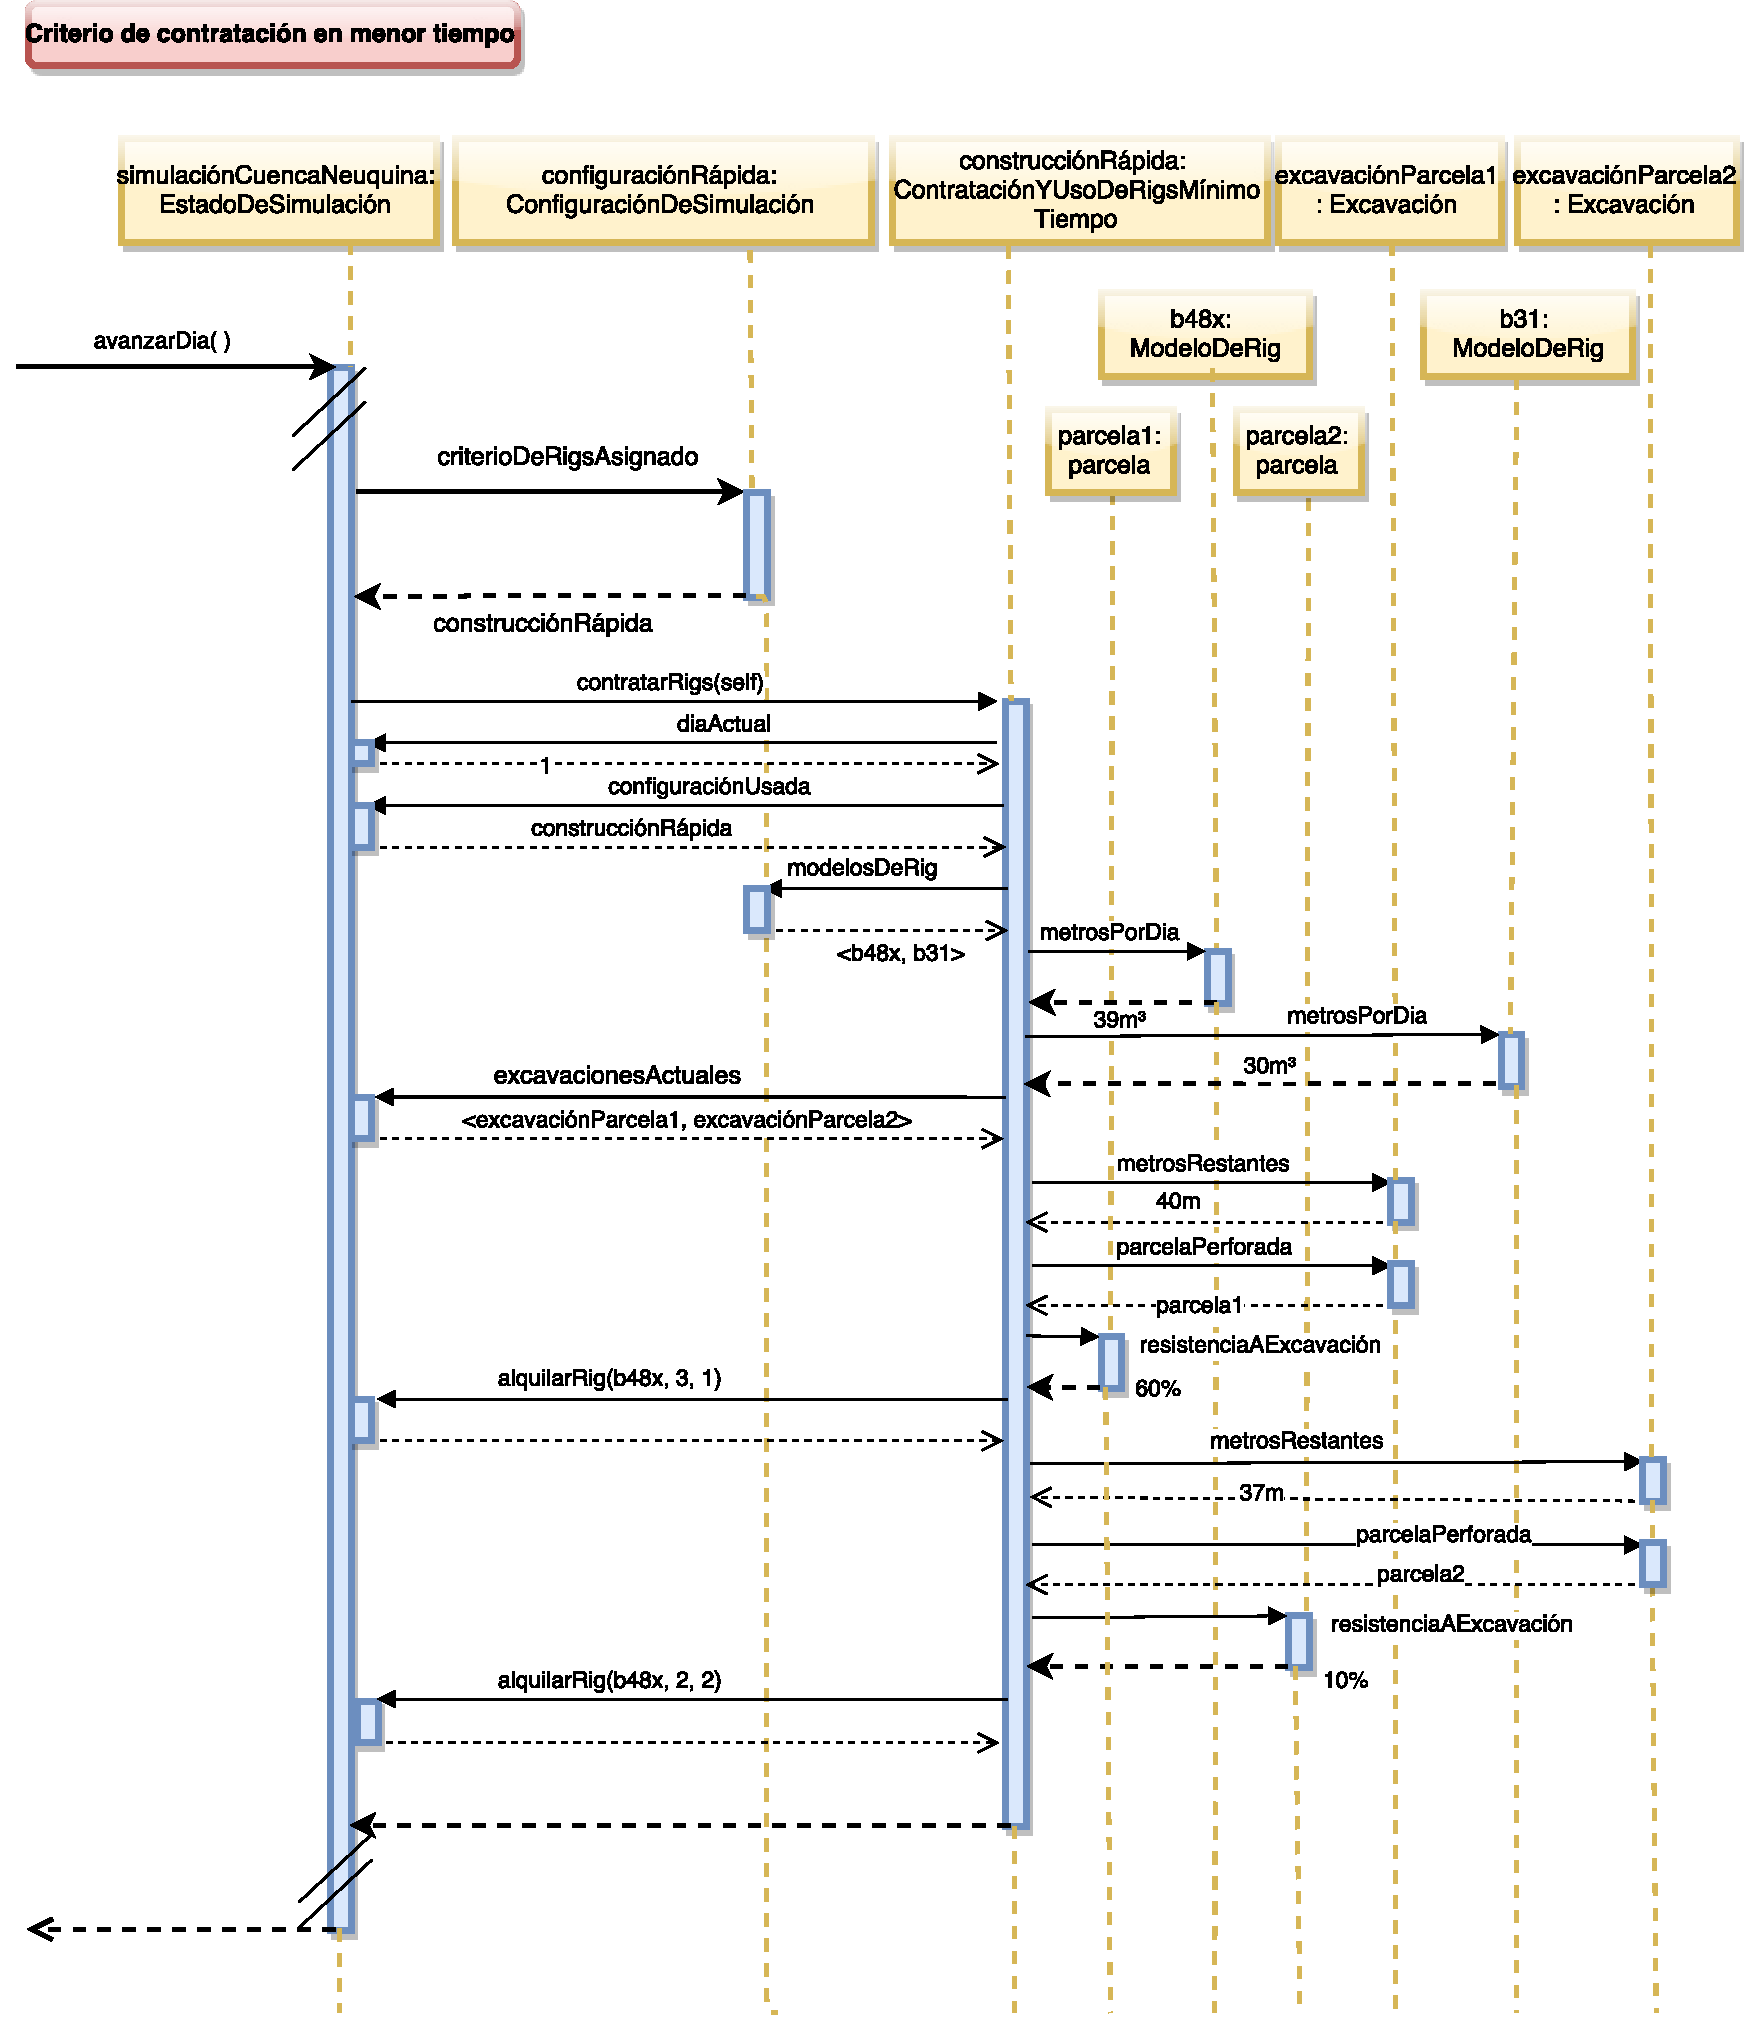
\includegraphics[width=1\textwidth, keepaspectratio]{rigs}
\end{figure}

Al igual que el criterio de construcción de plantas, el criterio de contratación se encarga de hacer todas las contrataciones necesarias el primer día. El resto de los días no contrata.
\\

Sabiendo el modelo de rig con más poder de excavación, el criterio de mínimo tiempo calcula cuántos días se necesitan para terminar de excavar todas las parcelas con este tipo de rig. De esta manera, las excavaciones terminan en el menor tiempo posible (aunque posiblemente alquilando los rigs más costosos).
\\

El mismo criterio luego responde al mensaje excavar simplemente asignando cualquiera de estos rigs con máximo poder de excavación a cada excavación existente (por la manera en que se contrata, siempre hay tantos rigs como excavaciones).
\\

En la versión de mínimo costo, se usa un único rig con menor costo final (es decir, ponderando consumo de combustible, costo de alquiler y días mínimos de alquiler) para realizar todas las excavaciones, aumentando tiempo pero también disminuyendo costos.

%%%%%%%%%%%%%%%%%%%%%%%%%%%%%%%%%%%%%%%%%%%%%%%%%

\newpage
\textbf{Diagrama de elección de parcelas}
\begin{figure}[H]
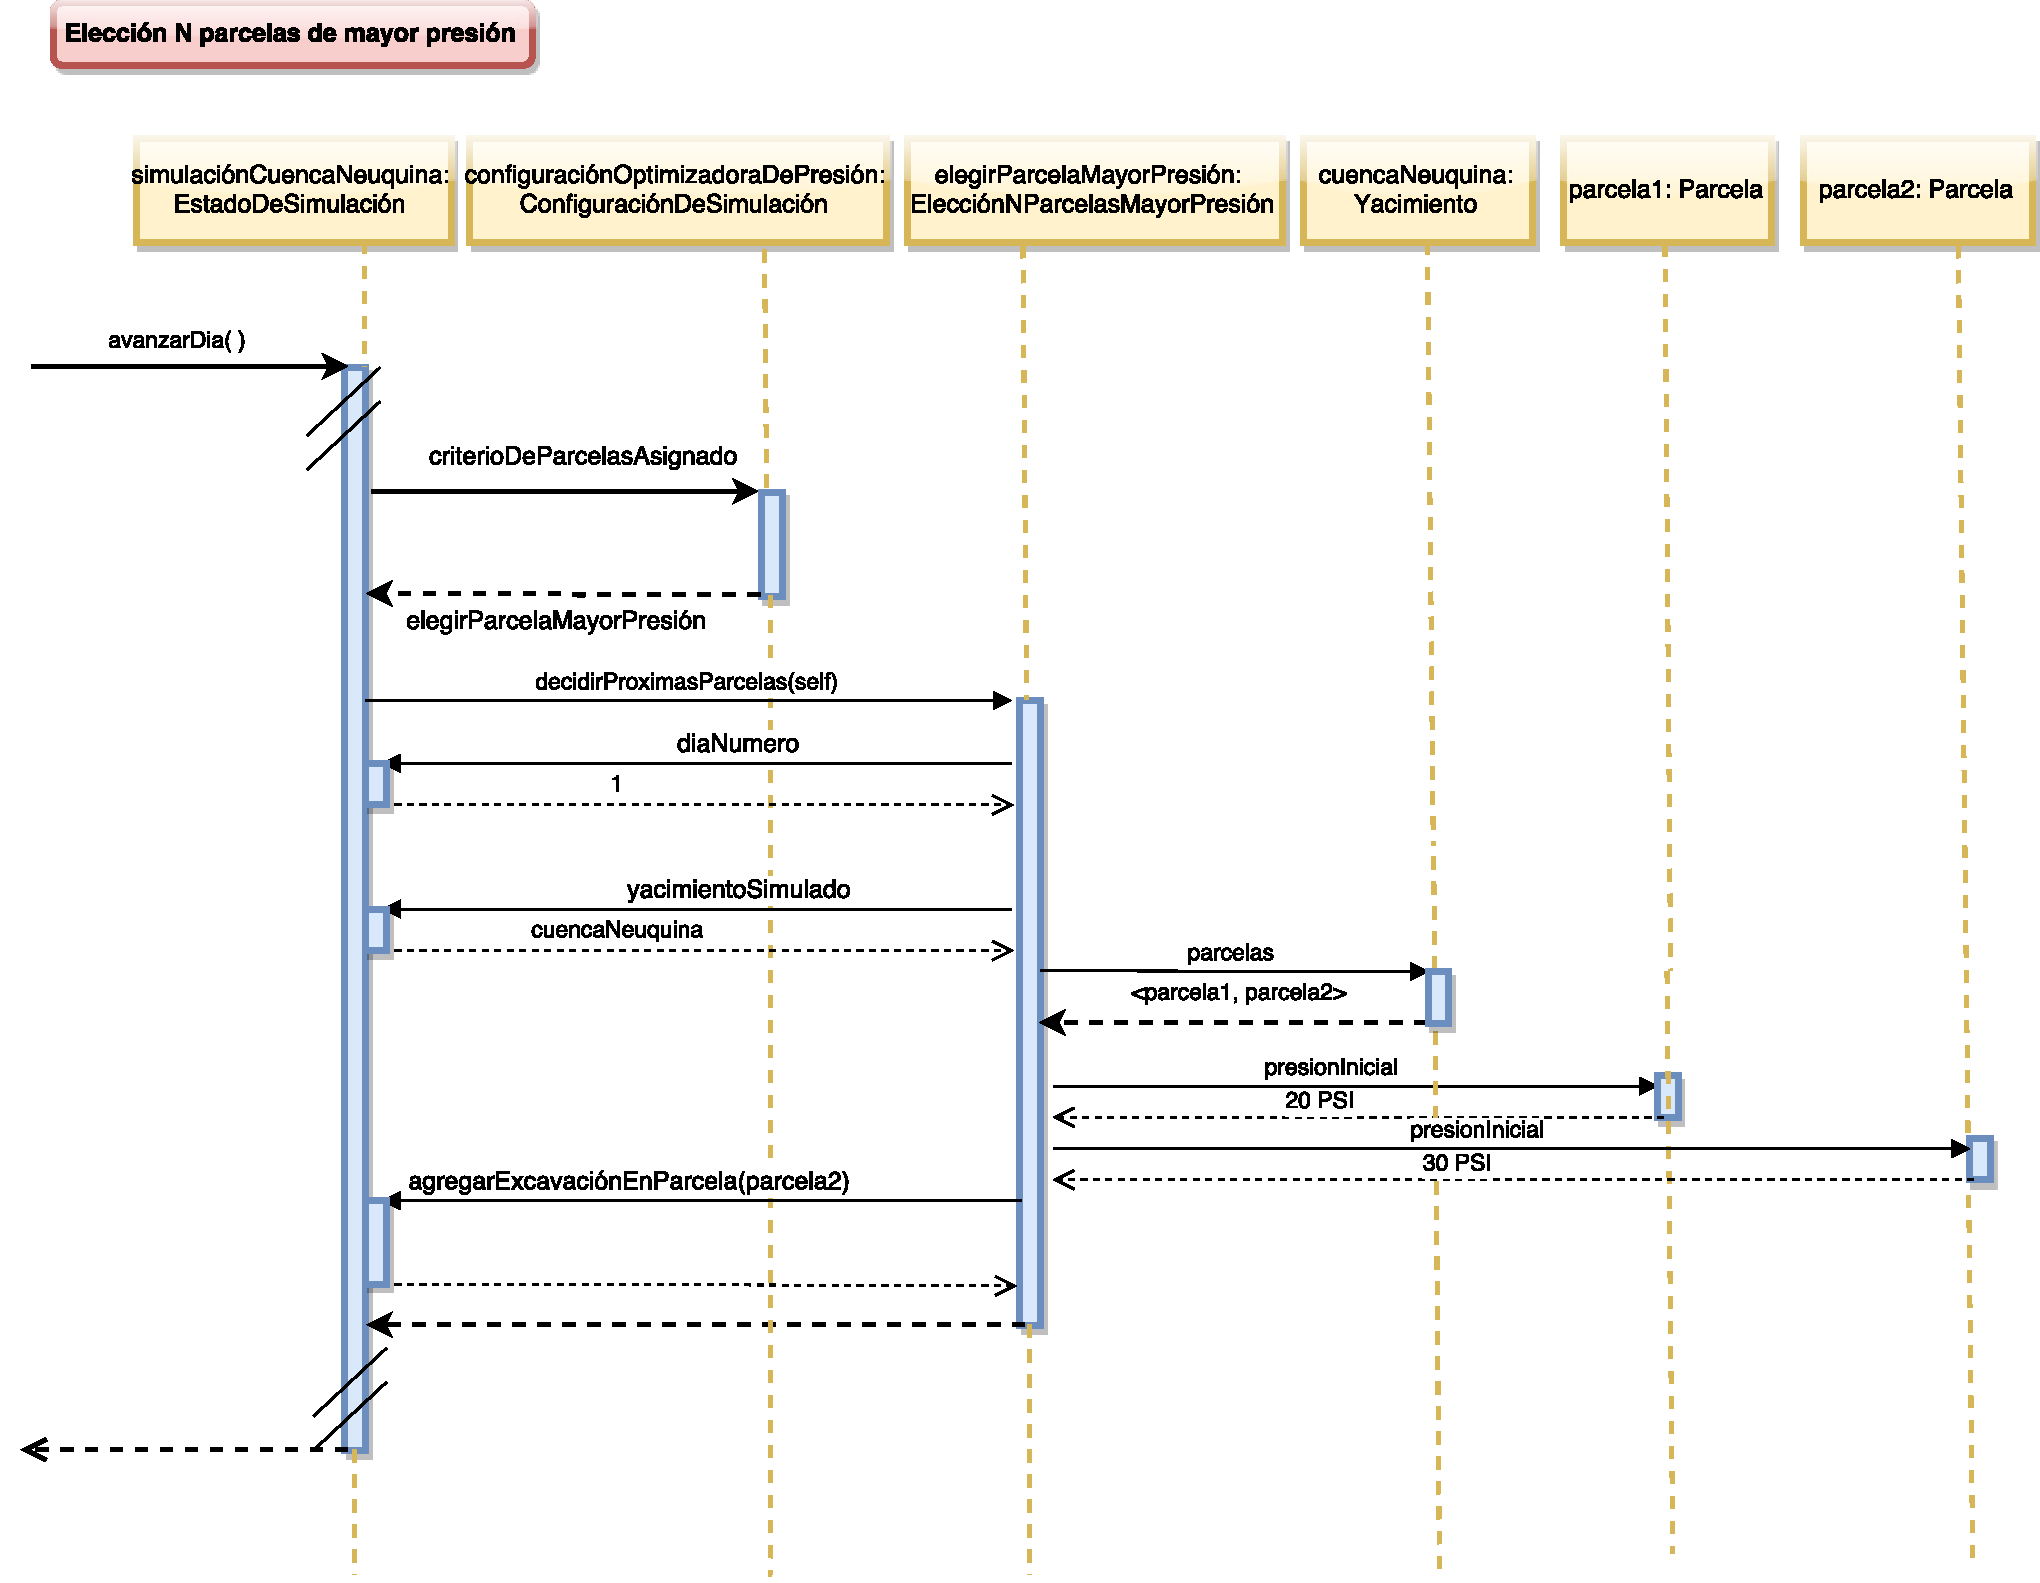
\includegraphics[width=1.15\textwidth, keepaspectratio]{parcelas}
\end{figure}

Cuando el estado de simulación llama al mensaje de decisión de las próximas parcelas a excavar el primer día, el criterio se encarga de consultar por el yacimiento simulado y, luego, por las parcelas que tiene. En el escenario del diagrama el criterio elige por mayor presión y la cantidad de parcelas elegibles prefijadas es 1, por lo tanto elige de las dos parcelas del yacimiento la parcela 2, que tiene mayor presión.
\\

En el caso del criterio que escoge N parcelas por profundidad, en lugar de preguntar por la presión inicial pregunta por la profundidad y escoge las N menores.
\\

Dado que el criterio elige el primer día la cantidad necesaria para el desarrollo de la explotación, el resto de los días no realiza nada en particular al recibir el mensaje.
\\

%%%%%%%%%%%%%%%%%%%%%%%%%%%%%%%%%%%%%%%%%%%%%%%%%

\newpage
\textbf{Diagrama de habilitación y extracción de pozos}
\begin{figure}[H]
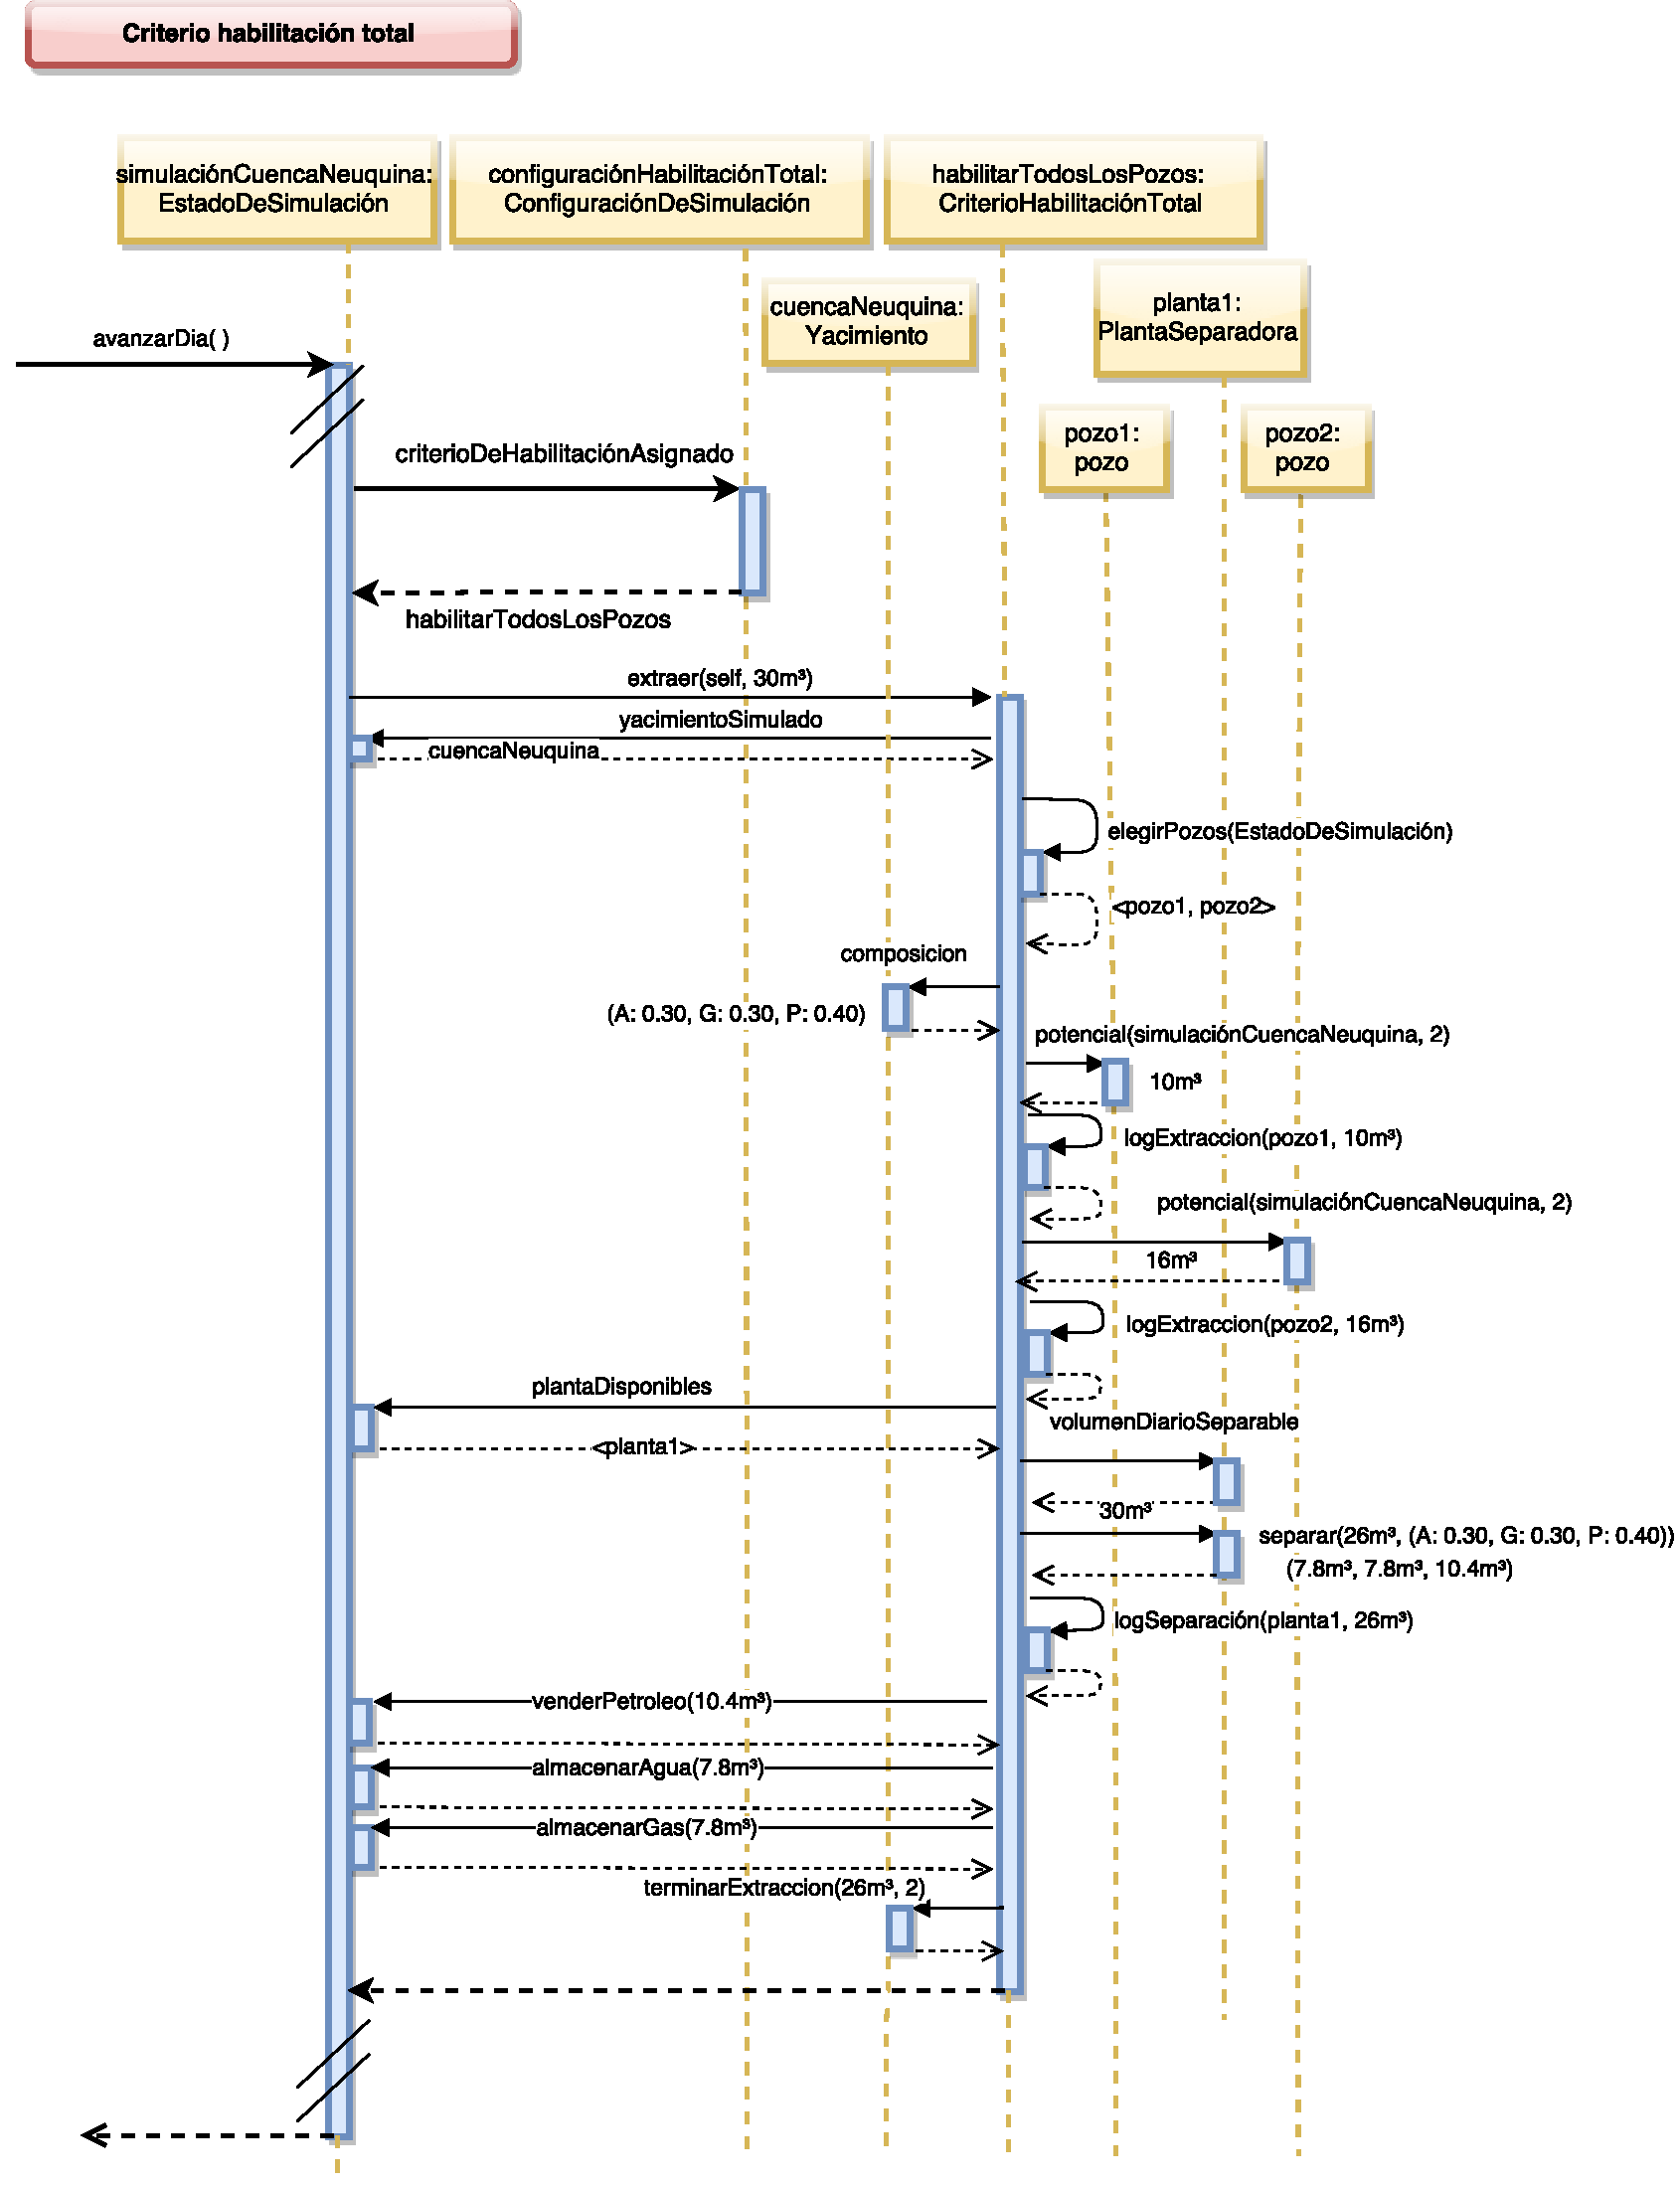
\includegraphics[width=0.9\textwidth, keepaspectratio]{extraccion}
\end{figure}

Cuando el estado envía el mensaje \emph{extraer} al criterio de habilitación de pozos este último consulta al primero por el yacimiento simulado para conocer su composición (lo conoce porque se envía como self junto con el tope de volumen extraíble).
\\

El tope de volumen el estado lo calcula sabiendo tanto el volumen separable (conocimiento que consigue de sus plantas) y almacenable tanto de agua y gas (conocimiento que consigue de sus tanques y de la composición del yacimiento) de modo que todo lo extraído sea tanto separable como almacenable (ni el gas ni el agua se pueden tirar).
\\

También se autoenvía el mensaje \emph{elegirPozos} (el cual a diferencia de \emph{extraer} es implementado por cada criterio en particualar) para saber cuáles son los pozos que tiene que iterar consultando por su potencial volumen. Por ser un criterio de habilitación total, elige los únicos dos pozos de la explotación. Si fuera la versión de N pozos de mayor presión, por ejemplo con N=1, hubiera elegido el pozo de los dos que mayor presión tuviera.
\\

Luego, conociendo las plantas del estado, se iteran para separar el total del producto extraído y finalmente indicandole al estado que venda el petróleo extraído y que almacene la cantidad de agua y gas extraída.
\\

Finalmente el criterio le indica al yacimiento que termine la extracción actualizando las presiones según la cantidad de pozos que se habilitó y el volumen que se extrajo.

%%%%%%%%%%%%%%%%%%%%%%%%%%%%%%%%%%%%%%%%%%%%%%%%%
